
\documentclass[12pt]{article}

\usepackage[bottom=3cm]{geometry}
\usepackage{p4doc}
\usepackage{fleqn}
\usepackage{fancyvrb}
\usepackage{graphicx}
\usepackage{tabularx}
\usepackage{soul}
\usepackage{float}
\usepackage{underscore}
\usepackage{tablefootnote}
\usepackage[table]{xcolor}

\usepackage[parfill]{parskip}

\usepackage{silence}
\WarningFilter{Fancyhdr}{\headheight is too small}
\WarningFilter{latex}{Overfull \hbox}


%%not_a_keyword auto
%%not_a_keyword default

%%not_a_keyword ternary
%%not_a_keyword exact
%%not_a_keyword lpm

%%not_a_keyword length

%%not_a_keyword type

%%not_a_keyword reads
%%not_a_keyword actions
%%not_a_keyword min_size
%%not_a_keyword max_size
%%not_a_keyword size
%%not_a_keyword modifier
%%not_a_keyword support_timeout


\lstdefinestyle{BNFstyle}{
    language=BNF,%
    frame=single,%
    backgroundcolor=\color{bnfgreen},%
    morekeywords={const_value, unsigned_value, bool_value, binary_value, decimal_value, hexadecimal_value, binary_base, hexadecimal_base, binary_digit, decimal_digit, hexadecimal_digit, width_spec, field_value, type_spec, data_type, object_ref, general_expr, bool_expr, arith_expr, bin_op, un_op, bool_op, rel_op, header_type_declaration, header_dec_body, field_dec, length_bin_op, length_exp, header_instance_declaration, header_instance, scalar_instance, array_instance, metadata_instance, metadata_initializer, header_ref, index, field_ref, field_list_declaration, field_list_entry, field_list_calculation_declaration, calculated_field_declaration, update_verify_spec, update_or_verify, if_cond, calc_bool_cond, value_set_declaration, parser_function_declaration, parser_function_body, parser_body_call, extract_statement, header_extract_ref, header_extract_index, set_statement, return_statement, return_value_type, case_entry, value_list, case_return_value_type, value_or_masked, select_exp, field_or_data_ref, parser_exception_declaration, return_or_drop, return_to_control, counter_declaration, counter_type, direct_or_static, direct_attribute, static_attribute, meter_declaration, meter_type, register_declaration, width_or_layout, width_declaration, layout_declaration, attribute_list, attr_entry, register_ref, primitive_action_declaration, simple_param_list, compound_action_function_declaration, action_param_list, action_param, param_qualifier, action_statement, arg_list, action_profile_declaration, action_specification, action_selector_declaration, table_declaration, field_match, field_or_masked_ref, field_match_type, table_actions, action_specification, action_profile_specification, control_function_declaration, control_block, control_statement, apply_call, apply_and_select_block, case_list, action_case, action_or_default, hit_miss_case, hit_or_miss, if_else_statement, else_block, extern_type_declaration, member_declaration, method_declaration, method_param_list, method_param, attribute_declaration, identifier_list, attribute_type, extern_instance_declaration, extern_attribute_binding, extern_method_call, p4_program, p4_declaration}%
}

\lstdefinestyle{P4style}{
    language=C,%
    frame=single,%
    backgroundcolor=\color{codeblue},%
    keywords={action, action_function_declaration, action_profile, action_selector, algorithm, and, apply, attribute, attributes, bit, bytes, calculated_field, control, counter, direct, direct_attibute, dynamic_action_selection, else, extern, extern_type, extract, false, field_list, field_list_calculation, fields, header, header_type, hit, if, in, inout, input, instance_count, int, last, layout, mask, max, metadata, meter, method, min, min_width, miss, next, not, optional, or, output_width, packets, parse_error, parser, parser_drop, parser_exception, parser_value_set, primitive_action, range, register, result, return, saturating, select, selection_key, set_metadata, signed, static, table, true, update, valid, value, varbit, verify, width},%
    basicstyle=\ttfamily,%
    aboveskip=3mm,%
    belowskip=3mm,%
    fontadjust=true,%
    keepspaces=true,%
    keywordstyle=\bfseries,%
    captionpos=b,%
    framerule=0.3pt,%
    firstnumber=0,%
    numbersep=1.5mm,%
    numberstyle=\tiny,%
}

\ifpdf
    \pdfinfo {
        /Author   (The P4 Language Consortium)
        /Title    (The P4 Language Specification, v 1.1.0)
        /Keywords (P4)
        /Subject  ()
        /Creator  (TeX)
        /Producer (PDFLaTeX)
    }
\fi

\begin{document}
\vspace{2cm}

%\title{\sffamily\bfseries\huge The P4 Language Specification\\ \vspace{3mm} \Large Version 1.0.2}
\centerline{\sffamily\bfseries\huge The P4 Language Specification}
\vspace{3mm}
\centerline{\sffamily\Large Version 1.1.0}
\vspace{3mm}
\centerline{\sffamily\large November 6, 2015}
\vspace{8mm}
\centerline{\sffamily\large The P4 Language Consortium}

\date{November 6, 2015}
\thispagestyle{firstpagestyle}
%\maketitle

%%%%%%
%%%%%%
\SECTION{Introduction}{intro}
%%%%%%
%%%%%%

P4 is a declarative language for expressing how packets are processed by the 
pipeline of a network forwarding element such as a switch, NIC, router or 
network function appliance. It is based upon an abstract forwarding model 
consisting of a parser and a set of \matchaction table resources, divided 
between ingress and egress. The parser identifies the headers present in 
each incoming packet. Each \matchaction table performs a lookup on a subset 
of header fields and applies the actions corresponding to the first match 
within each table. Figure 1 shows this model.

P4 itself is protocol independent but allows for the expression of forwarding 
plane protocols. A P4 program specifies the following for each forwarding 
element.

\begin{itemize}
\item
\textit{Header definitions:} the format (the set of fields and their
sizes) of each header within a packet.
\item
\textit{Parse graph:} the permitted header sequences within packets.
\item
\textit{Table definitions:} the type of lookup to perform, the input
fields to use, the actions that may be applied, and the dimensions of
each table.
\item
\textit{Action definitions:} compound actions composed from a set of
primitive actions.
\item
\textit{Pipeline layout and control flow:} the layout of tables within
the pipeline and the packet flow through the pipeline.
\end{itemize}


P4 addresses the configuration of a forwarding element. Once configured, tables 
may be populated and packet processing takes place. These post-configuration 
operations are referred to as "run time" in this document. This does not preclude 
updating a forwarding element's configuration while it is running.
\SUBSECTION{The P4 Abstract Model}{absmod}

The following diagram shows a high level representation of the P4 abstract 
model.

\begin{figure}[h!]
    \centering
    \includegraphics[width=\textwidth]{figures/p4\string_abs\string_model.png}
    \caption{Abstract Forwarding Model}
    \label{fig:abstractmodel}
\end{figure}

The P4 machine operates with only a few simple rules. 

\begin{itemize}
\item
For each packet, the parser produces a \textit{Parsed Representation}
on which \matchaction tables operate.
\item
The \matchaction tables in the \textit{Ingress Pipeline} generate an
\textit{Egress Specification }which determines the set of ports (and
number of packet instances for each port) to which the packet will be
sent.
\item
The \textit{Queuing Mechanism} processes this Egress Specification,
generates the necessary instances of the packet and submits each to
the \textit{Egress Pipeline}.  Egress queuing may buffer packets when
there is over-subscription for an output port, although this is not
mandated by P4.
\item
A packet instance's physical destination is determined before entering
the \textit{Egress Pipeline}.  Once it is in the Egress Pipeline, this
destination is assumed not to change (though the packet may be dropped
or its headers further modified).
\item
After all processing by the Egress Pipeline is complete, the packet
instance's header is formed from the Parsed Representation (as
modified by \matchaction processing) and the resulting packet is
transmitted.
\end{itemize}


Although not shown in this diagram, P4 supports recirculation and cloning 
of packets.  This is described in detail in Section~\ref{sec:recirc}.

P4 focuses on the specification of the parser, \matchaction tables and the 
control flow through the pipelines. Programmers control this by writing a 
P4 program which specifies the switch configuration as shown at the top of 
Figure 1. 

A machine that can run a P4 program is called \textit{target}. Although a target 
may directly execute a P4 program, it is assumed in this document that the 
program is compiled into a suitable configuration for the target.

In the current version, P4 does not expose, for example, the functionality 
of the Queuing Mechanism and does not specify the semantics of the Egress 
Specification beyond what is mentioned above. Currently they are defined in 
target specific input to the compiler and exposed in conjunction with other 
interfaces that provide run time system management and configuration. Future 
versions of P4 may expose configuration of these mechanisms allowing consistent 
management of such resources from the P4 program.

\SUBSECTION{The mTag Example}{mtag}

The original P4 paper [1] includes an example called mTag. We use this example 
throughout this specification as a means of explaining the basic language 
features as they are presented. Complete source for this example, including 
sample run time APIs, is available at the P4 web site [2].

We give an overview of the mTag example here.  Quoting from the original paper:

\begin{quote}
Consider an example L2 network deployment with top-of-rack (ToR) switches 
at the edge connected by a two-tier core. We will assume the number of end-hosts 
is growing and the core L2 tables are overflowing. . . .  P4 lets us express a 
custom solution with minimal changes to the network architecture. . . . The routes 
through the core are encoded by a 32-bit tag composed of four single-byte 
fields.  The 32-bit tag can carry a "source route".... Each core switch need 
only examine one byte of the tag and switch on that information. [1]
\end{quote}

Two P4 programs are defined for this example: One for edge switches (called 
"ToR" above) and one for aggregation switches (called "core switches" above). 
These two programs share definitions for packet headers, the parser and actions.

\SUBSECTION{Specification Conventions}{conventions}

This document represents P4 grammatical constructs using BNF with the
following conventions:

\begin{itemize}
\item
The BNF is presented in green boxes.
\item
Non-terminal nodes are indicated with \textbf{bold}.
\item
A node with a name ending in \texttt{_name} is implicitly a string whose first character 
is a letter (not a digit).
\item
Nodes followed by \texttt{+} indicate one or more instances.
\item
Nodes followed by \texttt{*} indicate zero or more instances.
\item
A vertical bar, \texttt{|}, separates options from which exactly one must be selected.
\item
Square brackets, \texttt{[]}, are used to group nodes. A group is optional unless 
it is followed by \texttt{+}. A group may be followed by * indicating zero or more 
instances of the group.
\item
Symbols with special significance (e.g., \texttt{[ ] * + |}) may be used as terminal 
nodes by enclosing them in quotes: for example "\texttt{*}".
\item
Symbols other than those listed above are literals. Examples include curly 
braces, colon, semi-colon, parentheses, and comma.
\item
If a rule does not fit on one line, a new line immediately follows \texttt{::=} and 
the description ends with a blank line.
\item
Example P4 code appears in blue boxes
\item
Example code in a language other than P4 appears in beige boxes
\end{itemize}

Header types and table definitions are specified declaratively.  These
typically consist of a set of attribute/value pairs separated by a
colon.

Parsers, actions and control flow are specified imperatively with
typed parameters (if any) and a limited set of operations.

%%%%%%
%%%%%%
\SECTION{Structure of the P4 Language}{structure}
%%%%%%
%%%%%%

\SUBSECTION{Abstractions}{p4abstractions}

P4 provides the following top-level abstractions: 

\begin{itemize}

\item
\textit{Base types:} Integers and bitstrings with arbitrary widths.
\item
\textit{Headers:}
\begin{itemize}
\item
\textit{Header types:} A specification of fields within a header.
\item
\textit{Header instances:} A specific instance of a packet header or metadata.
\end{itemize}
\item
\textit{Parser state function:} Defines how headers are identified
within a packet.
\item
\textit{Action function:} A composition of primitive actions that are to be applied 
together.
\item
\textit{Table instance:} Specified by the fields to match and the permitted actions.
\item
\textit{Control flow function:} Imperative description of the table application
order. 
\item
\textit{Stateful memories:} Counters, meters and registers which persist across packets.
\item
\textit{Extern:}
\begin{itemize}
\item
\textit{Extern types:} An object type provided by a standard library 
or target provider which can perform functionality not otherwise expressible
in P4.
\item
\textit{Extern instances:} A specific instance of an extern type.
\end{itemize}

\end{itemize}

In addition to these high level abstractions, the following are used

\begin{itemize}

\item
For a header instance:
\begin{itemize}
\item
\textit{Metadata:} Per-packet state which may not be derived from
packet data. Otherwise treated the same as a packet header.
\item
\textit{Header stack:} a contiguous array of header instances.
\item
\textit{Dependent fields:} Fields whose values depend on a calculation
applied to other fields or constants.
\end{itemize}

\item
For a parser:
\begin{itemize}
\item
\textit{Value set:} run-time updatable values used to determine parse
state transitions.
\item
\textit{Checksum calculations:} The ability to apply a function to a
set of bytes from the packet and test that a field matches the
calculation.
\end{itemize}

\end{itemize}


\SUBSECTION{Value Specifications}{valuespec}

P4 supports generic and bit-width specific values. These are unified through
the following representation.

%%bnf
\begin{lstlisting}[style=BNFstyle]
const_value ::=
    bool_value |
    [ "+" | - ] [ width_spec ] unsigned_value

unsigned_value ::= 
    binary_value | 
    decimal_value | 
    hexadecimal_value

bool_value ::= true | false
binary_value ::=  binary_base binary_digit+
decimal_value ::= decimal_digit+
hexadecimal_value ::= hexadecimal_base hexadecimal_digit+

binary_base ::= 0b | 0B
hexadecimal_base ::= 0x | 0X

binary_digit ::= _ | 0 | 1
decimal_digit ::= binary_digit | 2 | 3 | 4 | 5 | 6 | 7 | 8 | 9
hexadecimal_digit ::= 
    decimal_digit | a | A | b | B | c | C | d | D | e | E | f | F

width_spec ::= decimal_digit+ [ w | s ]
field_value ::= const_value
\end{lstlisting}
%%endbnf

The width specification is followed by a letter \texttt{w} or \texttt{s} 
depending on the sign of the value. The width must be specified in decimal.

Note that constants always start with a digit to distinguish them from other 
identifiers.

The node \texttt{const_value} may be read as 'constant value'. The node
\texttt{field_value} is used in this specification to emphasize that the width
of the representation may be relevant; otherwise it is a synonym for
\texttt{const_value}.

Whitespace terminates a constant specification.

Underscores are permitted in values to add clarity by grouping digits; they are
ignored otherwise. Examples include: \texttt{78_256_803} (replacing commas in
decimal representation) or \texttt{0b1101_1110_0101} (grouping bits into nibbles
or bytes in binary representation).

Negative numbers are represented in two's complement.  See
Section~\ref{sec:p4casting} for the P4 typing rules.

Here are some example values.

\begin{table}[H]
\begin{center}
\begin{tabular}{| l | l | l | p{.5\textwidth} |} \hline
\textbf{Notation} &
\textbf{Decimal Value} & 
\textbf{Bit Width} &
\textbf{Notes} \\ \hline
\texttt{42} &
42 &
6 &
Default base is decimal \\ \hline
\texttt{16w42} &
42 &
16 &
The same value, but explicitly given a width of 16 bits. \\ \hline
\texttt{0b101010} &
42 &
6 &
Binary representation of 42  \\ \hline
\texttt{12w0x100} &
256 &
12 &
Example of bit width and hexadecimal base indication. \\ \hline
\texttt{7w0b1} &
1 &
7 &
Binary value specified with explicit width \\ \hline
\texttt{-0B101} &
-5 &
4 &
\\ \hline
\end{tabular}
\end{center}
\caption{Value Representation Examples}
\end{table}

\SUBSECTION{Types and declarations}{p4types}

A P4 program consists of concrete declarations of the abstractions listed in
Section~\ref{sec:p4abstractions}.

Object declarations occur at the top-level of the program; declarations cannot 
happen conditionally, such as inside a specific parse state or branch of a 
control flow. Declarations consist of a type, as specified in the grammar below, 
followed by a unique identifier and an object body. The exact format of the 
body depends on the object type, and is described in more detail for each type 
throughout this document.

The order that objects are declared in does not matter, and objects can
reference other objects that were declared before them in the code.

P4 types generally consist of the kind of abstraction, followed by the specific
type name.


%%bnf
\begin{lstlisting}[style=BNFstyle]

type_spec ::=
    header [ header_type_name ] |
    metadata [ header_type_name ] |
    field_list |
    field_list_calculation |
    parser |
    parser_exception |
    parser_value_set |
    counter |
    meter |
    register |
    action |
    action_profile |
    table |
    control |
    extern [ extern_type_name ] |
    data_type

data_type ::=
    bit |
    bit < decimal_digit+ > |
    varbit < decimal_digit+ > |
    int < decimal_digit+ >
\end{lstlisting}
%%endbnf

P4 actions consist of signatures which look like the typed
parameter lists of traditional programming languages. The types of the
parameters in these signatures must be one of the above.

The \textit{bit} type represents a bitstring of the length specified within
angle brackets (a compile time constant). If the angle brackets are omitted, the
length is implied to be 1. Most of the data processed by P4 is stored in a
bitstring of some sort, as described in Section~\ref{sec:p4casting}.

The \textit{varbit} type represents a bitstring with a length that is variable
at run time, but \textit{at most} the length specified within angle brackets
(again, a compile time constant). This data type is used for quickly parsing
through variable-length headers and does not currently have utility beyond
that. More functionality may be added for this type in subsequent versions of P4
(such as the ability to read it from a \matchaction pipeline).

Types which are followed by an optional identifier like \textit{header} can be 
used in two ways:
\begin{itemize}
\item
    "\texttt{header foo}" refers to a header instance specifically of
    header_type \textit{foo}
\item
    "\texttt{header}" without an identifier refers to any header instance,
    of \textit{any} type.
\end{itemize}

\SUBSECTION{P4 data types}{p4casting}

\newtoggle{conditionalExpression}
\togglefalse{conditionalExpression}

\newcommand{\code}[1]{\texttt{#1}}
\newcommand{\bool}{\code{\textbf{bool}}}
\newcommand{\infint}{\code{\textbf{int}}}
\newcommand{\W}{\code{\emph{W}}}
\newcommand{\Wone}{\code{\emph{W1}}}
\newcommand{\bit}[1]{\code{\textbf{bit}<#1>}}
\newcommand{\Int}[1]{\code{\textbf{int}<#1>}}
\newlength{\descwidth}
\setlength{\descwidth}{12cm}

P4 is a strongly-typed language; all values are statically
typed. Programs that do not pass type-checking are invalid.

P4 supports several base types and allows the construction of derived
types.  This section discusses only the following base types: Booleans
and types for representing integers (bitstrings).

\SUBSUBSECTION{Principles}{typing-principles}

The typing rules for the integer types are chosen according to the
following principles:

\begin{description}
\item[Inspired from C:] Typing of integers is modeled after the
  well-defined parts of C, expanded to cope with arbitrary fixed-width
  integers.  In particular, the type of the result of an expression
  only depends on the expression operands, and not on how the result
  of the expression is consumed.
\item[No undefined behaviors:] P4 attempts to remedy the undefined C
  behaviors.  Unfortunately C has many undefined behaviors, including
  specifying the size of an integer (\code{int}), results produced on
  overflow, and results for some arguments values (e.g., shifts with
  negative amounts, division of negative numbers, overflows on signed
  numbers, etc.).  In contrast, P4 computations on integer types have
  \emph{no undefined behaviors}.
\item[Least surprise:] The P4 typing rules are chosen to behave as
  closely as possible to traditional well-behaved C programs.
\item[Forbid rather than surprise:] Rather than provide surprising or
  undefined results (e.g., in C comparisons between signed and
  unsigned integers), we have chosen to forbid expressions with
  ambiguous interpretations.  For example, P4 does not allow binary
  operations that combine signed and unsigned integers.
\end{description}

The priority of arithmetic operations is also chosen similar to C
(e.g., multiplication binds stronger than addition).

\SUBSUBSECTION{Base types}{typing-base-types}

The P4 base types are shown in Table~\ref{tab:summary}.

\begin{table}[!h]
  \center
  \begin{tabular}{|lp{6.5cm}ll|} \hline
    \textbf{Type} & \textbf{Description} & \textbf{Example} &
    \textbf{Section} \\ \hline
    
    \bool & Boolean values & \bool & \ref{sec:bool} \\ 
    \bit{\W} & Fixed-width unsigned integers of an arbitrary width~\W &
    \bit{20} & \ref{sec:unsigned} \\
    \Int{\W} & Fixed-width signed integers of an arbitrary width~\W,
    represented using two's complement & \Int{33} & \ref{sec:signed} \\
    \code{\textbf{varbit}<\W>} & Bit-strings of dynamically-computed width
    (also called \emph{varbits}) with a
    maximum width~\W & \code{\textbf{varbit}<1024>} & \ref{sec:varbit} \\
    \code{\textbf{int}} & Infinite-precision integer constant values & \infint &
    \ref{sec:integer} \\

    \hline
  \end{tabular}
  \caption{Base P4 Types\label{tab:summary}}
\end{table}

Values can be converted to a different type by using casts.  The range
of casts available is intentionally restricted.  There are very few
implicit casts.  Most binary operations require both operands to be of
the same type.  No operations produce runtime exceptions.

\SUBSUBSECTION{Portability}{typing-portability}

No P4 target can support all possible types and operations.  For
example, the following type is legal in P4: \bit{23132312}.
Hence, each target can impose restrictions on the values it can support.
Such restrictions may include:

\begin{itemize}
\item The maximum width supported
\item Alignment and padding constraints (e.g., arithmetic may only be
  supported on widths which are an integral number of bytes).
\item Constraints on some operands (e.g., some architectures may only
  support multiplications with small constants, or shifts with small
  values).
\end{itemize}

Target-specific documentation should describe such restrictions, and
target-specific compilers should provide clear error messages when
such restrictions are encountered.  An architecture may reject a
well-typed P4 program and still be conformant to the P4 spec.
However, if an architecture accepts a P4 program as valid, the runtime
program behavior should match this specification.

\SUBSUBSECTION{No saturated types}{typing-saturated}

P4 does not support saturated integer types for the following reasons:

\begin{itemize}
\item Saturated types are unlikely to be portable.
\item The semantics of many operations on saturated types may be open
  for debate.
\item Most operations may be unnecessary on saturated types (addition,
  subtraction and multiplication seem to be the most frequent ones).
\item Finally, saturated arithmetic can be implemented by using P4
  v1.1 \code{extern} custom constructs that operate on bitstrings
  rather than by built-in arithmetic operators.  For example, an
  architecture could provide an \code{extern saturated\_alu} whose
  methods operate on unsigned bitstrings but perform saturated
  operations.
\end{itemize}

\SUBSUBSECTION{Boolean\label{sec:bool}}{typing-boolean}

The Boolean type contains two values, \code{\textbf{false}} and
\code{\textbf{true}}.  The type is written as \bool.  Operations on
Boolean values are described in Section~\ref{sec:booloperations}.
Booleans are not integers.

\SUBSUBSECTION{Unsigned integers (bit-strings)}{unsigned}

An unsigned integer (which we also call a ``bit-string'') has an
arbitrary width, expressed in bits.  A bit-string of width \W{} is
declared as: \bit{\W}.  \W{} must be a compile-time constant value
evaluating to a positive integer greater than 0.

Bits within a bit-string are numbered from 0 to \W-1.  Bit 0 is the
least significant, and bit \W-1 is the most significant\footnote{No P4
  operation currently depends on the bit numbering within an integer,
  but future language additions may.}.

For example, the type \bit{128} denotes the type of bit-string
values with 128 bits numbered from 0 to 127, where bit 127 is the most
significant.

The type \code{\textbf{bit}} is a shorthand for \bit{1}.

P4 target architectures may impose additional compile-time or runtime
constraints on \code{bit} types: for example, they may limit the
maximum size, or they may only support some arithmetic operations on
certain sizes (e.g., 16-, 32- and 64- bit values).

All operations that can be performed on unsigned integers are
described in Section~\ref{sec:unsignedoperations}.

\SUBSUBSECTION{Signed Integers}{signed}

Signed integers are represented using 2's complement.  An integer with
\W{} bits is declared as: \Int{\W}.  \W{} must be a compile-time
constant value evaluating to a positive integer greater than 0.

Bits within an integer are numbered from 0 to \W-1. Bit 0 is the least
significant, and bit \W-1 is the sign bit.

For example, the type \Int{64} describes the type of integers
represented using exactly 64 bits.

There are no constraints of the value of \W, but specific targets may
impose limits.

All operations that can be performed on signed integers are
described in Section~\ref{sec:signedoperations}.

\SUBSUBSECTION{Dynamically-sized bit-strings}{varbit}

Some network protocols use fields whose size is only known at runtime
(e.g., IPv4 options). To support restricted manipulations of such
values, P4 provides a special bit-string type whose size is set at
runtime, called a varbit.

\code{\textbf{varbit}<\W>} denotes a bit-string with a width of
\emph{at most} \W{} bits, where \W{} is a compile-time constant value
evaluating to a positive integer.  For example, the type
\code{\textbf{varbit}<120>} denotes the type of bit-string values that
may have between 0 and 120 bits.  Most operations that are applicable
to fixed-size bit-strings (unsigned numbers) cannot be performed on
dynamically sized bit-strings.

P4 target architectures may impose additional compile-time or runtime
constraints on \code{\textbf{varbit}} types: for example, they may limit the
maximum size, or they may require \code{\textbf{varbit}} values to always
contain an integer number of bytes at runtime.

All operations that can be performed on dynamically-sized bitstrings
are described in Section~\ref{sec:varbitoperations}.

\SUBSUBSECTION{Infinite-precision integers}{integer}

The infinite-precision datatype describes integers with an unlimited
precision.  This type is written as \infint.  This type is reserved
for compile-time integer literals only.  No P4 run-time value can have
an \infint{} type; at compile time the compiler will convert all
\infint{} values that have a runtime component to fixed-width types,
according to the rules described below.

All operations that can be performed on infinite-precision integers
are described in Section~\ref{sec:intoperations}.

\SUBSUBSECTION{Integer literal types}

As described in Section~\ref{sec:valuespec}, there are three types of integer
literals (constants):

\begin{itemize}
\item A simple integer constant has type \infint.
\item A simple positive integer can be prefixed with a width and the
  character 'w'  (no spaces) to indicate an unsigned integer with the
  specified width in bits.
\item A simple integer (positive or negative) can be prefixed with a
  width and the character 's' (no spaces) to indicate a signed integer
  with the specified width in bits.
\end{itemize}

Table~\ref{tab:literals} shows several examples of integer literals
and their types.

\begin{table}[!h]
  \center
    \begin{tabular}{|rl|} \hline
      \textbf{Literal} & \textbf{Interpretation} \\ \hline
      \code{10} & Type is \infint, value is 10. \\
      \code{-10} & Type is \infint, value is -10. \\
      \code{8w10} & Type is \bit{8}, value is 10. \\
      \code{8w-10} & Illegal: negative unsigned number. \\
      \code{8s10} & Type is \Int{8}, value is 10. \\
      \code{8s-10} & Type is \Int{8}, value is -10. \\
      \code{2s3} & Type is \Int{2}, value is -1 (last 2 bits), overflow warning. \\
      \code{1w10} & Type is \bit{1}, value is 0 (last bit), overflow warning. \\
      \code{1s10} & Type is \Int{1}, value is 0 (last bit), overflow warning. \\
      
      \hline
    \end{tabular}
  \caption{Integer literals and their types.\label{tab:literals}}
\end{table}

\SUBSECTION{Base type operations}{typing-operations}

This section describes all legal operations that can be performed on
base types.  For each operation we describe the input operand types
and the result type.

\SUBSUBSECTION{Computations on Boolean values}{booloperations}

\textbf{Note:} In C binary Boolean operations are performed using
short-circuit evaluation, where the second operand is only evaluated
if necessary.  This is important only if the evaluation of an operand
can produce side-effects.  Currently there are no operations in P4
that produce side-effects.  In consequence, there is no semantic
difference between short-circuit and full evaluation.  If the P4
language is extended in the future to encompass operations with
side-effects, the semantics of Boolean operations may have to be
revisited.

Table~\ref{tab:booloperations} describes all operations available on
Boolean values.

\begin{table}[!h]
  \center
  \begin{tabular}{|lp{\descwidth}|} \hline
    \textbf{Operation} & \textbf{Description} \\ \hline
    \code{\textbf{and}}\tablefootnote{We propose replacing the keyword
      \code{\textbf{and}} with the equivalent C operator \code{\&\&} in a
      future P4 revision.} & Binary associative operation; both
    operands must be Boolean; result is Boolean. \\

    \code{\textbf{or}}\tablefootnote{We propose replacing the keyword \code{\textbf{or}} with
      the equivalent C operator \code{||} in a future P4 revision.}
    & Binary associative operation; both operands must be Boolean;
    result is Boolean. \\
    
    \code{\textbf{not}}\tablefootnote{We propose replacing the keyword \code{\textbf{not}}
      with the equivalent C operator \code{!} in a future P4
      revision.} & Unary operation; operand is Boolean, result is
    Boolean. \\

    \code{==}, \code{!=} & Test for equality/inequality; result is
    Boolean. \\

    \hline
  \end{tabular}
  \caption{Boolean operations\label{tab:booloperations}}
\end{table}

In addition, all comparison operations (\code{==}, \code{!=},
\code{>}, \code{<}, \code{<=}, \code{>=}), described below, produce as
results Boolean values.

There are no implicit casts from bit-strings to Booleans or
vice-versa.  In consequence, a C program fragment such as: \\
\code{if (x) ... } \\
(for \code{x} an integer base type) must be written in P4 as: \\
\code{if (x != 0) ... } \\
(see also the discussion on infinite-precision types and implicit
casts~\ref{sec:implicitcasts} for how the 0 in this expression is
evaluated).

\iftoggle{conditionalExpression}{
\paragraph{The conditional expression} \mbox{}\\

We propose adding the P4 a conditional expression operator, similar to
C's ternary \code{?:} operator.  The \code{?:} expression behaves as
in C.  The first argument is Boolean, and the second and third
arguments must have the exact same type.
}

\SUBSUBSECTION{Operations on unsigned fixed-width integers}{unsignedoperations}

This section discusses all operations that can be performed on values
with \bit{\W} types.

Operations ``wrap-around'', similar to C operations on unsigned values
(i.e., representing a large value on \W{} bits will only keep the
least-significant \W{} bits of the value).  There are no arithmetic
exceptions; the runtime result of an arithmetic operation is defined
for all combinations of input arguments.

All binary operations (except shifts) require both operands to have
the same exact type and width; supplying operands with different
widths produces a compile-time error.  No implicit casts are inserted
by the compiler to equalize the widths.  There are no binary
operations that combine signed and unsigned values (except shifts).

Table~\ref{tab:unsignedoperations} shows all operations available on
  unsigned values.

\begin{table}[!h]
  \center
  \begin{tabular}{|lp{\descwidth}|} \hline
    \textbf{Operation} & \textbf{Description} \\ \hline

    \code{==}, \code{!=} & Test for equality/inequality.  Both
    operands must have the same width.  The result is a Boolean
    value. \\

    \code{<}, \code{>}, \code{<=}, \code{>=} & Unsigned comparisons.
    Both operands must have the same width.  The result is a Boolean
    value. \\
    
    \code{\&}, \code{|}, \verb|^| & Bitwise operations; both operands
    must have the same width; result is unsigned and has the same
    width.  \\
    
    \code{\~{}} & Result is unsigned and has the same width as the
    input.  Bitwise complement. \\

    \verb|<<|, \verb|>>| & Left operand is unsigned, right operand
    must be either an unsigned number or a non-negative constant
    integer.  The result has the same type as the left operand.  These
    perform logical shifts (fill with zero.)  Shifts with an amount
    greater or equal to the width of the input produce a result with
    all bits zero. \\

    \code{+} (unary) & Unary plus sign; behaves as a no-op. \\
    
    \code{-} (unary) & Unary negation; the result is computed by by
    subtracting its value from $2^\W$.  The result is always unsigned
    and it has the same width as the input.  The semantics is the same
    as the C negation of unsigned numbers. \\

    \code{+} (binary) & Binary addition; associative.  Both operands
    must have the same type; result has the same type.  Result is
    computed by truncating the result of the mathematical addition to
    the width of the output (similar to C). \\
    
    \code{-} (binary) & Binary subtraction; associative.  Both
    operands must have the same type; result is unsigned, and has the
    same type.  Result is computed by adding the negation of the
    second operand (similar to C). \\
    
    \code{*} & Binary unsigned multiplication; associative.  Both
    inputs must have the same width; result has the same width as
    the inputs, and is unsigned.  P4 targets may impose additional
    restrictions (e.g., may require one of the operands to be a
    compile-time constant value, or only allow multiplications with
    powers of two). \\
    
    \hline
  \end{tabular}
  \caption{Operations on unsigned values.\label{tab:unsignedoperations}}
\end{table}

There is no unsigned integer division operator.

\SUBSUBSECTION{Operations on signed fixed-width integers}{signedoperations}

This section discusses all operations that can be performed on
\Int{\W} types.  An \Int{\W} type is a signed integer with \W{} bits
represented using 2's complement.

``Underflow'' or ``overflow'' produced by arithmetic cannot be
detected: operations ``wrap-around'', similar to C operations on
unsigned values (i.e., representing a large value on \W{} bits will
only keep the least-significant \W{} bits of the value).  (Note that C
does not define the result of operations that overflow when computing
on signed values, whereas P4 does.)  There are no arithmetic
exceptions; the runtime result of an arithmetic operation is defined
for all combinations of input arguments.

All binary operations (except shifts) require both operands to have
the same exact type (signedness) and width; supplying operands with
different widths or signedness produces a compile-time error.  No
implicit casts are inserted by the compiler to equalize the widths.
there are no binary operations that combine signed and unsigned values
(except shifts).

Table~\ref{tab:signedoperations} shows all operations available on
signed values.

\begin{table}[!h]
  \center
  \begin{tabular}{|lp{\descwidth}|} \hline
    \textbf{Operation} & \textbf{Description} \\ \hline
    \code{==}, \code{!=} & Test for equality/inequality.  Both
    operands must have the same width.  The result is a Boolean
    value. \\

    \code{<}, \code{>}, \code{<=}, \code{>=} & Signed comparisons.
    Both operands must have the same width.  The result is a Boolean
    value. \\
    
    \code{\&}, \code{|}, \verb|^| & Bitwise operations; both operands
    must have the same width; result is signed and has the same width. \\
    
    \code{\~{}} & Result is signed and has the same width as the
    input.  Bitwise complement. \\

    \verb|<<|, \verb|>>| & Left operand is signed, right operand must
    be either an unsigned number or a non-negative constant integer.
    The result has the same type as the left operand.  These perform
    arithmetic shifts.  Shifts with an amount greater or equal to the
    width of the input are allowed. \\

    \code{+} (unary) & Unary plus sign; behaves as a no-op. \\
    
    \code{-} (unary) & Unary negation; the result is signed and it
    has the same width as the input. \\

    \code{+} (binary) & Binary addition; associative.  Both operands
    must have the same type; result has the same type.  \\
    
    \code{-} (binary) & Binary subtraction; associative.  Both
    operands must have the same type; result is signed, and has
    the same type.  \\
    
    \code{*} & Binary signed multiplication; associative.  Both
    inputs must have the same width; result has the same width as
    the inputs, and is signed.  P4 targets may impose additional
    restrictions (e.g., may require one of the operands to be a
    compile-time constant value, or only allow multiplications with
    powers of two). \\
    
    \hline
  \end{tabular}
  \caption{Operations on signed values.\label{tab:signedoperations}}
\end{table}

Note that bitwise operations are well-defined, since the
representation is mandated to be 2's complement.

There is no signed integer division operator.

\SUBSUBSECTION{A note about shifts}{typing-shifts}

Shifts (on signed and unsigned values) deserve a special discussion,
due to the following reasons:

\begin{itemize}
  \item As in C, right shift behaves differently for signed and
    unsigned values: right shift for signed values is an arithmetic
    shift.
  \item Shifting with a negative amount does not have a clear
    semantics: while in C the result is undefined, in P4 the type
    system makes it illegal to shift with a negative amount.
  \item In C, shifting with an amount larger or equal to the number of
    bits has an undefined result (unlike our definition).
  \item Finally, shifting may require doing work which is exponential
    in the number of bits of the right-hand-side operand.  Consider
    the following examples:

%%code
\begin{lstlisting}[style=P4style]
bit<8> x;
bit<16> y;
... y << x ...
... y << 1024 ...
\end{lstlisting}
%%endcode
    
    Unlike C, P4 gives a precise meaning shifting with an amount
    larger than the size of the shifted value.
\end{itemize}

Due to these reasons, P4 targets may impose additional restrictions to
shift operations:

\begin{itemize}
\item Targets may reject shifts by non-constant amounts.
\item Targets may reject shifts with large non-constant amounts.  For
  example, a target may forbid shifting an 8-bit value by a value
  wider than 3 bits.
\end{itemize}

\SUBSUBSECTION{\code{varbit} operations}{varbitoperations}

The type \code{\textbf{varbit}<\W>} denotes variable-size bitstrings (varbit)
with a maximum static width of \W{} bits.  Such a bit-string has a
\emph{dynamic} width, which must be smaller or equal than \W.  Prior
to initialization a varbit has a dynamic width of 0.  Varbits support
a limited set of operations:

\begin{itemize}
\item Parser extraction into a varbit. This operation sets the dynamic
  width of the value.  The extracted value must be shorter than the
  static width \W.
\item deparsers can use the emit method to insert the contents of a
  varbit into a packet.
\end{itemize}

There are no arithmetic, comparisons, bit-wise, or bit extraction
operators on varbits.  If these are desired, \code{\textbf{varbit}} types
should not be used.

\SUBSUBSECTION{Operations on arbitrary-precision integers}{intoperations}

The type \infint{} denotes integer values on which computations are
performed with arbitrary precision.  Table~\ref{tab:intoperations}
shows all operations that are defined for \infint{} values.  The only
values that can have the type \infint{} are compile-time constants.

All the operands that participate in an operation must have type
\infint{}; binary operations (except shift) cannot combine \infint{}
values with fixed-width types.  For such expressions the compiler will
always insert an implicit cast; this cast will always convert the
\infint{} value to the fixed-width type.

All computations on \infint{} values are carried without information
loss.  For example, multiplying two 1024-bit values may produce a
2048-bit value (note that concrete representation of \infint{} values
is not specified).

Casting an \infint{} value to a fixed-width type will preserve the
least-significant bits.  If the truncation causes significant bits to
be lost, the compiler should emit a suitable warning. 

\begin{table}[!h]
  \center
  \begin{tabular}{|lp{\descwidth}|} \hline
    \textbf{Operation} & \textbf{Description} \\ \hline

    \code{==}, \code{!=} & Test for equality/inequality.  Both
    operands must be \infint{}s.  The result is a Boolean value. \\

    \code{<}, \code{>}, \code{<=}, \code{>=} & Signed comparisons.
    Both operands must be \infint{}s.  The result is a Boolean
    value. \\
    
    \verb|<<|, \verb|>>| & Right operand must be a positive \infint.
    The result has the same type as the left operand.  $a$ \verb|<<|
    $b$ is $a \times 2^b$.  $a$ \code{>>} $b$ is $\lfloor a /
    2^b\rfloor$ (expressed using real-number division). \\

    \code{+} (unary) & Unary plus sign; behaves as a no-op. \\
    
    \code{-} (unary) & Unary negation; the result is an \infint; no
    information is lost in negation. \\

    \code{+} (binary) & Binary addition; associative.  Both operands
    must be \infint; result is \infint, and no information is lost in
    addition (no overflow). \\
    
    \code{-} (binary) & Binary subtraction; associative.  Both
    operands must be \infint; result is \infint; no information is
    lost in subtraction (no overflow).  \\
    
    \code{*} & Binary signed multiplication; associative.  Both
    inputs must be \infint; result is \infint.  No overflow
    occurs. \\

    \code{/, \%} & Binary signed division and modulo.  Both inputs
    must be positive \infint{} values; result is a positive \infint{}
    value. \\

    \hline
  \end{tabular}
  \caption{Operations on arbitrary-precision constant
    integers.\label{tab:intoperations}}
\end{table}

Note: bitwise-operations (\code{|}, \code{\&}, \verb|^|, \code{\~{}})
are \emph{not} defined for \infint{} values.  Division and modulo are
illegal for negative values (the C language does not give a clear
semantics to division of signed integers when values are negative).

\SUBSECTION{Casts}{typing-casts}

\SUBSUBSECTION{Explicit casts}{typing-explicit-casts}

P4 supports a very limited range of casts.  Most casts must be
explicit.  Most binary operations require both operands to have the
exact same type.  Some type conversions may require multiple chained
casts.  While more onerous for the user, this approach has several
benefits:

\begin{itemize}
\item Makes user intent unambiguous.  
\item Makes the conversion cost explicit.  Some casts involve
  sign-extensions, and thus require significant computational
  resources.
\item Reduces the number of cases that have to be considered in the P4
  specification.
\end{itemize}

A cast expression is written as in C, \code{(typeRef)exp}, where
\code{typeRef} is a reference to a type (e.g., a type name).

All legal casts are shown in table~\ref{tab:casts}.

\begin{table}[!h]
  \center
  \begin{tabular}{|llp{\descwidth}|} \hline
    \textbf{From} & \textbf{To} & \textbf{Description} \\ \hline

    \bit{1} & \bool & 0 is false, 1 is true \\
    \bool & \bit{1} & reverse of the above \\
    \bit{\W} & \Int{\W} & Preserves all bits unchanged \\
    \Int{\W} & \bit{\W} & Preserves all bits unchanged \\

    \bit{\W} & \bit{\Wone} & if \W $\geq$ \Wone{} this keeps
    least-significant \Wone{} bits, if \W $<$ \Wone{} this causes
    extension with zero bits \\
    
    \Int{\W} & \Int{W1} & if \W $\geq$ \Wone{} this keeps least-significant
    \Wone{} bits, if \W $<$ \Wone{} this causes extension with the sign
    bits \\

    \infint & \bit{W} & Represents the integer value using two's
    complement on a large enough number of bits and keeps the
    least-significant \W{} bits; overflow should lead to a warning,
    including conversion of a negative number \\

    \infint & \Int{W} & Represents the integer value using two's
    complement on a large enough number of bits and keeps the
    least-significant \W{} bits; overflow should lead to a warning \\
    
    \hline
  \end{tabular}
  \caption{Legal P4 casts.\label{tab:casts}}
\end{table}

\SUBSUBSECTION{Implicit casts}{implicitcasts}

Unlike C, P4 allows a very limited number of implicit casts.  The
reason is that often the implicit casts have a non-trivial semantics,
which is invisible for the programmer.  Implicit casts are allowed in
P4 only when their meaning is completely unambiguous:

\begin{itemize}
\item To convert an \infint{} value to a fixed-width type.
\item In assignments (including passing arguments to method calls),
  when RHS has a different type from LHS.
\end{itemize}

Most binary operations that take an \infint{} and a fixed-width
operand will insert an implicit cast to convert the \infint{} operand to
the type of the fixed-width operand.

Consider a program with the following values:

%%code
\begin{lstlisting}[style=P4style]
bit<8>  x;
bit<16> y;
int<8>  z;
\end{lstlisting}
%%endcode

Table~\ref{tab:implicit} shows how implicit casts are inserted by the compiler:

\begin{table}[!h]
  \center
  \begin{tabular}{|ll|} \hline
    \textbf{Expression} & \textbf{Implementation} \\ \hline
    
    \code{x+1} & \code{x+(\bit{8})1} \\

    \code{z<0} & \code{z<(\Int{8})0} \\

    \iftoggle{conditionalExpression}{
    \code{(x==0)?y:0} & \code{(x==(\bit{8})0)?y:(\bit{16})0} \\
    }
    
    \code{x<{}<13} & \code{0}; overflow warning \\

    \code{x|0xFFF} & \code{x|(\bit{8})0xFFF}; overflow warning \\
    
    \hline
  \end{tabular}
  \caption{Examples of implicit casts.\label{tab:implicit}}
\end{table}

\SUBSUBSECTION{Illegal expressions}{typing-illegal}

Consider a program with the following values:

%%code
\begin{lstlisting}[style=P4style]
bit<8>  x;
bit<16> y;
int<8>  z;
\end{lstlisting}
%%endcode

Table~\ref{tab:illegal} shows several expressions which are illegal
because they do not obey the P4 typing rules.  For each expression we
provide several ways that the expression could be manually rewritten
into a legal expression.  Note that for some expression there are
several legal alternatives, which may produce different results!

\begin{table}[!h]
  \center
  \begin{tabular}{|lll|} \hline
    \textbf{Expression} & \textbf{Why is it illegal} & \textbf{Alternatives} \\ \hline

    \code{x+y} & Different widths & \code{(\bit{16})x+y} or \\
               &                  & \code{x+(\bit{8})y} \\ \hline

    \code{x+z} & Different signs  & \code{(\Int{8})x+z} or \\
               &                  & \code{x+(\bit{8})z} \\ \hline
           
    \code{(\Int{8})y} & Cannot change both size and width & \code{(\Int{8})(\bit{8})y} or  \\
               &         & \code{(\Int{8})(\Int{16})y} \\ \hline

    \code{y+z} & Different widths and signs & \code{(\Int{8})(\bit{8})y+z} or \\
               &                  & \code{y+(\bit{16})(\bit{8})z} or \\
               &                  & \code{(\bit{8})y+(\bit{8})z} or \\
               &                  & \code{(\Int{16})y+(\Int{16})z} \\ \hline

    \code{x<{}<z} & RHS of shift cannot be signed & \code{x<{}<(\bit{8})z} \\ \hline

    \iftoggle{conditionalExpression}{
    \code{x?y:0} & First operand must be \bool & \code{(x!=0)?y:0} \\ \hline
    }
    
    \code{x<z}  & Different signs & \code{x<(\bit{8})z} or \\
                &                 & \code{(\Int{8})x<z} \\ \hline
    
    \code{1<{}<x} & Width of 1 unknown & \code{((\bit{32})1)<{}<x} or \\
                &                 & \code{32w1<{}<x} \\ \hline

    \code{\~{}1}   & Bitwise operation on \infint & \code{\~{}32w1} \\ \hline

    \code{5\&-3} & Bitwise operation on \infint & \code{32w5\&-3} \\
    
    \hline
  \end{tabular}
  \caption{Illegal P4 expressions.\label{tab:illegal}}
\end{table}

\SUBSECTION{References}{p4refs}

Concrete instances of the above types are referenced via their instance names.  
P4 is lexically scoped.

%%bnf
\begin{lstlisting}[style=BNFstyle]
object_ref ::=
    instance_name |
    header_ref |
    field_ref
\end{lstlisting}
%%endbnf

The terminal \textit{instance_name} refers to any named object, while header 
and field references are handled specially as described in 
Section~\ref{sec:headerreferences}.

\SUBSECTION{Expressions}{p4expressions}

Various language constructs can contain expressions built out of these object
references.

%%bnf
\begin{lstlisting}[style=BNFstyle]

general_expr ::= 
    bool_expr | arith_expr | object_ref

bool_expr ::=
    valid ( object_ref ) | bool_expr bool_op bool_expr |
    not bool_expr | ( bool_expr ) | arith_expr rel_op arith_expr |
    bool_value

arith_expr ::=
    object_ref | value | 
    max ( arith_expr , arith_expr ) | min ( arith_expr , arith_expr ) |
    ( arith_expr ) | arith_expr bin_op arith_expr | un_op arith_expr |
    ( data_type ) arith_expr

bin_op ::= "+" | "*" | - | << | >> | & | "|" | ^
un_op ::= ~ | -
bool_op ::= or | and
rel_op ::= > | >= | == | <= | < | !=

\end{lstlisting}
%%endbnf

Operator precedence and associativity follows C programming conventions.

The \textit{min} and \textit{max} functions return whatever is the smaller or
larger of their two arguments, respectively, or the first argument if the two 
compare equally.

%%%%%%
%%%%%%
\SECTION{Headers and Fields}{hdrs}
%%%%%%
%%%%%%

\SUBSECTION{Header Type Declarations}{headertypes}

Header types describe the layout of fields and provide names for referencing 
information. Header types are used to declare header and metadata instances. 
These are discussed in the next section.

Header types are specified declaratively according to the following BNF:

%%bnf
\begin{lstlisting}[style=BNFstyle]
header_type_declaration ::= 
   header_type header_type_name { header_dec_body }

header_dec_body ::=
    fields { field_dec * }
    [ length : length_exp ; ]

field_dec ::= data_type field_name ;
length_bin_op ::= "+" | - | "*" | << | >>
length_exp ::=
    const_value |
    field_name |
    length_exp length_bin_op length_exp |
    ( length_exp )

\end{lstlisting}
%%endbnf

Header types are defined with the following conventions.
\begin{itemize}
\item
Header types must have a \texttt{fields} attribute. 
\begin{itemize}
\item
The list of individual fields is ordered.
\item
Fields must be either of type \textit{bit} or \textit{varbit}.
\item
The bit offset of a field from the start of the header is determined by the 
sum of the widths of the fields preceding it in the list.
\item
Bytes are ordered sequentially (from the packet ordering).
\item
Bits are ordered within bytes by most-significant-bit first.  Thus, if the 
first field listed in a header has a bit width of 1, it is the high order 
bit of the first byte in that header.
\item
All bits in the header must be allocated to some field.
\item
One field at most within a header type may be of type \textit{varbit}, which 
indicates it is of variable length.
\end{itemize}

\item
If all fields are fixed width (no fields of type \textit{varbit}) then the header is 
said to be of \textit{fixed length}. Otherwise it is of \textit{variable length}.
\item
The \texttt{length} attribute specifies an expression whose evaluation gives
the length  of the header in \textit{bytes} for variable length headers. 
\begin{itemize}
\item
It must be present if the header has variable length (some field has type  
\textit{varbit}).
\item
A compiler warning must be generated if it is present for a fixed length header.
\item
Fields referenced in the length attribute must be located before the variable 
length field.
\end{itemize}
\item
If, at run time, the calculated length results in more data extracted to
the \textit{varbit} than its declared maximum length a parser exception is
triggered. See Section~\ref{sec:parserexceptions}.

\item
Operator precedence and associativity follows C programming conventions.
\end{itemize}

An example declaration for a VLAN header (802.1Q) is:

%%code
\begin{lstlisting}[style=P4style]
header_type vlan_t {
    fields {
        bit<3>  pcp;
        bit     cfi;
        bit<12> vid;
        bit<16> ethertype;
    }
}
\end{lstlisting}
%%endcode

Metadata header types are declared with the same syntax.

%%code
\begin{lstlisting}[style=P4style]
header_type packet_metadata_t {
    fields {
        bit<16> ingress_port; // The port on which the packet arrived.

        bit<16> length;       // The number of bytes in the packet. 
                              // For Ethernet, does not include the CRC. 
                              // Cannot be used if the switch is in
                              // 'cut-through' mode.

        bit<8>  type;         // Represents the type of instance of
                              // the packet: 
                              //   - PACKET_TYPE_NORMAL
                              //   - PACKET_TYPE_INGRESS_CLONE
                              //   - PACKET_TYPE_EGRESS_CLONE
                              //   - PACKET_TYPE_RECIRCULATED
                              // Specific compilers will provide macros
                              // to give the above identifiers the
                              // appropriate values
    }
}
\end{lstlisting}
%%endcode

P4 supports variable-length packet headers via fields of type \textit{varbit}.
The width of such a field is inferred from the total header length (which
is in bytes) as indicated by the \texttt{length} attribute: \texttt{((8 *
length) - sum-of-fixed-width-fields)}. Only one field at most within a header
may specify a field of type \textit{varbit}.

An example of a variable-width header is IPv4 with options:

%%code
\begin{lstlisting}[style=P4style]
header_type ipv4_t {
    fields {
        bit<4> version;
        bit<4> ihl;
        bit<8> diffserv;
        bit<16> totalLen;
        bit<16> identification;
        bit<3> flags;
        bit<13> fragOffset;
        bit<8> ttl;
        bit<8> protocol;
        bit<16> hdrChecksum;
        bit<32> srcAddr;
        bit<32> dstAddr;
        varbit<320> options;
    }
    length : ihl * 4;
}
\end{lstlisting}
%%endcode

This header can be parsed and manipulated the same way fixed-length headers
are, with the exception that there are no language facilities to read or
write data in the \textit{options} field.

\SUBSECTION{Header and Metadata Instances}{headerinstances}

While a header type declaration defines a header \textit{type}, a packet may contain 
multiple instances of a given type.  P4 requires each header instance to 
be declared explicitly prior to being referenced. 

There are two sorts of header instances: packet headers and metadata. Usually, 
packet headers are identified from the packet as it arrives at ingress while 
metadata holds information about the packet that is not normally represented 
by the packet data such as ingress port or a time stamp.  

Most metadata is simply per-packet state used like scratch memory while
processing a packet. However, some metadata may have special significance to
the operation  of the forwarding element. For example, the queuing system may
interpret the value of a particular metadata field when choosing a queue for a
packet. P4 acknowledges these target specific semantics, but does not attempt
to represent them.

Packet headers (declared with the \texttt{header} keyword) and metadata (declared 
with the \texttt{metadata} keyword) differ only in their validity. Packet headers 
maintain a separate valid indication which may be tested explicitly. Metadata 
is always considered to be valid. This is further explained in 
Section~\ref{sec:testing}.  Metadata instances are 
initialized to 0 by default, but initial values may be specified in their 
declaration.

The BNF for header and metadata instances is:

%%bnf
\begin{lstlisting}[style=BNFstyle]
header_instance_declaration ::= header_instance | metadata_instance
header_instance ::= scalar_instance | array_instance
scalar_instance ::= header header_type_name instance_name ;
array_instance ::=
    header header_type_name 
        instance_name "[" const_value "]" ;

metadata_instance ::= 
   metadata header_type_name
       instance_name [ metadata_initializer ] | ;

metadata_initializer ::= { [ field_name : field_value ; ] + }
\end{lstlisting}
%%endbnf


Some notes:

\begin{itemize}
\item
Only packet headers (not metadata instances) may be arrays (header stacks).
\item
\texttt{header_type_name} must be the name of a declared header type.
\item
Metadata instances may not be declared with variable length header types.
\item
The fields named in the initializer must be from the header type's \texttt{fields} list.
\item
If an initializer is present, the named fields are initialized to the indicated 
values; unspecified values are initialized to 0.
\item
The total length of all fields in a header instance must be an integral number
of bytes. The compiler may produce an error or insert padding at the end of
the header to resolve this issue.
\item
Only packet headers (not metadata instances) may be arrays (header stacks).
\end{itemize}


For example:

%%code
\begin{lstlisting}[style=P4style]
header vlan_t inner_vlan_tag;
\end{lstlisting}
%%endcode

This indicates that space should be allocated in the Parsed
Representation of the packet for a \texttt{vlan_t} header. It may be
referenced during parsing and \matchaction by the name
\texttt{inner_vlan_tag}.

A metadata example is:

%%code
\begin{lstlisting}[style=P4style]
metadata global_metadata_t global_metadata;
\end{lstlisting}
%%endcode

This indicates that an \texttt{global_metadata_t} type object called
\texttt{global_metadata} should be allocated for reference during
\matchaction.  

\SUBSUBSECTION{Testing if Header and Metadata Instances are Valid}{testing}

Packet headers and their fields may be checked for being
\textit{valid} (that is, having a defined value). Validity and
deparsing (see Section~\ref{sec:deparsing}) are the only points where packet
headers and metadata headers differ.

A header instance, declared with the keyword \texttt{header}, is \textit{valid}
if it is extracted during parsing (see Section~\ref{sec:parser}) or if an action
makes it valid (add or copy). A field (inside a header instance) is valid if its
parent header instance is valid.

All fields in a metadata instance are always valid.  Testing a
metadata field for validity should raise a compiler warning and will
always evaluate to True.

\begin{adjustwidth}{1.5cm}{1.5cm}
\textbf{Explanation: } The reason for this is best seen by examining
the case of a "flag"; for example, suppose a one bit metadata flag is
used to indicate that a packet has some attribute (say, is an IP
packet, v4 or v6).  There is no practical difference between the flag
having a value of 0 and the flag itself being invalid.  Similarly,
many "index" metadata fields can be given a reserved value to indicate
they are invalid (hence support for initial values of metadata
fields).  While occasionally it would be useful to have an independent
valid bit for a metadata field, defining a separate metadata flag to
represent that field's validity is a reasonable work around.
\end{adjustwidth}

Only valid packet header fields may result in a match (when a value is
specified for exact or ternary matches against the field), although a
match operation may explicitly check if a header instance (or field)
is valid. Only valid packet headers are considered for deparsing (see
Section~\ref{sec:deparsing}).  

\SUBSUBSECTION{Header Stacks}{headerstacks}

P4 supports the notion of a \textit{header stack} which is a sequence of
adjacent headers of the same type. MPLS and VLAN tags are examples that might
be treated this way.  Header stacks are declared as arrays as shown in
Section~\ref{sec:headerinstances}, and are of fixed length. Adding or removing
elements from the stack does not change the number of headers in the array - it
just changes the number of \textit{valid} headers in the array.

Header stack instances are referenced using bracket notation and such
references are equivalent to a non-stack instance reference. Each
element in the stack has its own validity bit. The following special
indices can be used to reference variable locations in the stack:

\begin{itemize}
\item
\textit{last}: The largest-index element that is \textit{valid}.
Used primarily to refer the higher-indexed end of the stack in \matchaction.
\item
\textit{next}: The smallest-index element that is \textit{invalid}.
Used primarily for parsing header data into a stack in a loop.
\end{itemize}

The special primitive actions \texttt{push()} and \texttt{pop()} are used to add 
and remove headers from the stack inside a \matchaction table. See Section~\ref{sec:xxx} 
for more details.

\SUBSECTION{Header and Field References}{headerreferences}

For match, action and control flow specifications, we need to make
references to header instances and their fields. Headers are
referenced via their instance names.  For header stacks, an index is
specified in square brackets. The keyword \texttt{last} can be used as an
index to refer to the largest-index valid instance of a header stack, while
\texttt{next} refers to the smallest-index \textit{invalid} instance.

Dotted notation is used to refer to a particular field inside of a header
instance. 

%%bnf
\begin{lstlisting}[style=BNFstyle]
header_ref ::= header_instance_name | header_instance_name "[" index "]"
index ::= const_value | last | next

field_ref ::= header_ref . field_name
\end{lstlisting}
%%endbnf

For example \texttt{inner_vlan_tag.vid} where
\texttt{inner_vlan_tag} has been declared as an instance of header
type \texttt{vlan_tag}.

\begin{itemize}
\item
Field names must be listed in the \texttt{fields} attribute of the
header declaration.
\item
A field reference is always relative to its parent header.  This allows the 
same field name to be used in different header types without ambiguity.
\item
Each header instance may be valid or invalid at any given time. This state 
may be tested in \matchaction processing.
\item
References at run time to a header instance (or one of its fields) which is 
not valid results in a special ``undefined'' value.  The implications of this 
depend on the context.
\end{itemize}

\SUBSECTION{Field Lists}{fieldlists}

In many cases, it is convenient to specify a sequence of fields. For example, 
a hash function may take a sequence of fields as input or a checksum may be 
calculated based on a sequence of fields.  P4 allows such declarations. Each 
entry may be a specific field instance reference, a header instance (which 
is equivalent to listing all the header's fields in order) or a fixed value. 
Packet headers and metadata may be referenced in a field list.

%%bnf
\begin{lstlisting}[style=BNFstyle]
field_list_declaration ::=
    field_list field_list_name {
        [ field_list_entry ; ] *
    }

field_list_entry ::= 
    object_ref | field_value
\end{lstlisting}
%%endbnf

The objects referenced in a field list must be either header instances,
fields, or other field lists. Recursive field list references are not
supported.

%%%%%%
%%%%%%
\SECTION{Checksums and Hash-value generators}{checksandhash}
%%%%%%
%%%%%%

Checksums and hash value generators are examples of functions that operate on a
stream of bytes from a packet to produce an integer. These have many
applications in networking. The integer may be used, for example, as an
integrity check for a packet or as a means to generate a pseudo-random value in
a given range on a packet-by-packet or flow-by-flow basis.

P4 provides a means of associating a function with a set of fields and
allowing the resulting operation (a map from packets to integers) to
be referenced in P4 programs.  These are called field list
calculations or calculation objects.  P4 does not support the
expression of the algorithm for computing the underlying function,
treating these like primitive actions. A set of known algorithms are
identified for convenience.

The resulting functions -- a field list calculation maps a packet to
an integer -- may be configurable through run time APIs. Targets may
vary in their support of these interfaces, but typically the seed
value of the calculation may be configured, the algorithm may have
configurable parameters (such as the coefficients for a polynomial
used in the calculation) and possibly even the set of fields used may
be configured.

The field list may be referenced as a field property for checksums,
discussed in Section~\ref{sec:checksums}, or referenced in a primitive action.

%%bnf
\begin{lstlisting}[style=BNFstyle]
field_list_calculation_declaration ::=
    field_list_calculation field_list_calculation_name {
        input {
            [ field_list_name ; ] +
        }
        algorithm : stream_function_algorithm_name ;
        output_width : const_value ;
    }
\end{lstlisting}
%%endbnf

Run time APIs allow the selection of one of the input field lists to
be active at a time. The first listed name is used as the default.

The \texttt{output_width} value is in bits.

A field instance is excluded from the calculation (i.e., it is treated as 
if the instance is not listed in the input list) if the field's header 
is not valid.

The algorithm is specified as a string.  The following algorithms are
defined with the given names, and targets may support others.

\begin{itemize}
\item
\textbf{xor16:} Simply the XOR of bytes taken two at a time.
\item
\textbf{csum16:} See the IPv4 header checksum description in \\
\url{https://tools.ietf.org/html/rfc791\#page-14}.
\item
\textbf{optional_csum16:} See the UDP header checksum description in \\
\url{https://tools.ietf.org/html/rfc768#page-2}.
\item
\textbf{crc16:} See \url{http://en.wikipedia.org/wiki/Crc16}.
\item
\textbf{crc32:} See \url{http://en.wikipedia.org/wiki/Crc32}
\item
\textbf{programmable_crc:}  This algorithm allows the specification 
of an arbitrary CRC polynomial.  See
\url{http://en.wikipedia.org/wiki/Cyclic_redundancy_check}.
\end{itemize}

\SUBSECTION{Checksums}{checksums}

Some fields, such as the IP checksum, hold the result of a stream
calculation.  P4 allows the representation of these dependencies with
the calculated field declaration. Calculated fields matter to the
extent they are verified at packet ingress or are updated at packet
egress.

The syntax associates a sequence of update or verify directives to a
specific field instance, each of which may have a condition associated
with it. The first entry with a condition satisfied by the packet (or
with no condition specified) determines the association. This
complexity allows the selection of different calculations based on the
packet's format. For example, the calculation of a TCP checksum may
vary slightly based on whether the packet has an IPv4 or an IPv6
header.

Note that the conditions are evaluated at the point the verify or
update operations are carried out.

Currently only limited conditions are supported.

%%bnf
\begin{lstlisting}[style=BNFstyle]
calculated_field_declaration ::=
    calculated_field field_ref { update_verify_spec + }

update_verify_spec ::=
    update_or_verify field_list_calculation_name [ if_cond ] ;

update_or_verify ::= update | verify
if_cond ::= if ( calc_bool_cond )
calc_bool_cond ::=
    valid ( header_ref | field_ref ) |
    field_ref == field_value
\end{lstlisting}
%%endbnf

Here is an example declaration. It assumes \texttt{field_list_calculation} declarations 
for \texttt{tcpv4_calc} and \texttt{tcpv6_calc} have been given and that \texttt{ipv4} and \texttt{ipv6} are 
packet header instances.

%%code
\begin{lstlisting}[style=P4style]
calculated_field tcp.chksum {
        update tcpv4_calc if (valid(ipv4));
        update tcpv6_calc if (valid(ipv6));
        verify tcpv4_calc if (valid(ipv4));
        verify tcpv6_calc if (valid(ipv6));
}
\end{lstlisting}
%%endcode

For checksums, the field list calculation is intended to bind the field list 
and algorithm to a specific field instance. This declaration indicates that 
the value stored in \texttt{field_ref} is expected to be the value calculated by the 
given field set calculation on the packet. Note that although this declaration 
may occur anywhere in the P4 program, the declaration \textbf{should} be placed immediately 
after the header instance declaration for the field referenced.

Fields with type \texttt{varbit} cannot be declared as calculated fields.

The \texttt{verify} option indicates that the parser should calculate the expected 
value and check if that value is stored in the indicated field. If the value 
is not equal, then a \texttt{p4_pe_checksum} exception is generated; see 6.6.1. 
Standard Parser Exceptions. This check occurs at the end of parsing and is 
performed only if \texttt{field_ref} is valid.

The \texttt{update} option indicates that the system should update the value of the 
field if changes are made to any fields on which it depends. The update to 
the field occurs when the packet is deparsed for egress. If no update clause 
applies, the field retains its value from the \matchaction pipeline.

%%%%%%
%%%%%%
\SECTION{Parser Specification}{parser}
%%%%%%
%%%%%%

P4 models the parser as a state machine. This can be represented as a parse 
graph with each state a node and the state transitions as edges. Figure 2 
shows a very simple example. Note that this figure identifies a header with 
each state. While P4 supports this approach, it does not require it. A node 
in the parse graph may be purely a decision node and not bound to a particular 
header instance, or a node may process multiple headers at once.

\begin{figure}[h!]
    \centering
    \includegraphics[width=\textwidth]{figures/parse\string_graphs.png}
    \caption{Simple Parse Graph and mTag Parse Graph}
    \label{fig:parsegraphs}
\end{figure}


Here are a few of the P4 parser functions for the mTag parser. The 
start function calls ethernet directly.

%%code
\begin{lstlisting}[style=P4style]
parser ethernet {
    extract(ethernet);   // Start with the ethernet header
    return select(latest.ethertype) {
        0x8100:     vlan;
        0x800:      ipv4;
        default:    ingress;
    }
}

parser vlan {
    extract(vlan);
    return select(latest.ethertype) {
        0xaaaa:     mtag;
        0x800:      ipv4;
        default:    ingress;
    }
}

parser mtag {
    extract(mtag);
    return select(latest.ethertype) {
        0x800:      ipv4;
        default:    ingress;
    }
}
\end{lstlisting}
%%endcode


The reference to \texttt{ingress} terminates parsing and invokes the ingress control 
flow function.

\SUBSECTION{Parsed Representation}{parsedreps}

The parser produces the representation of the packet on which \matchaction 
stages operate. This is called the \textit{Parsed Representation} of the packet. 
It is the set of header instances which are valid for the packet. The parser 
produces the initial Parsed Representation as described below. \Matchaction 
may update the Parsed Representation of the packet by modifying field values 
and by changing which header instances are valid; the latter results in adding 
and removing headers. 

The Parsed Representation holds packet headers as they are updated by \matchaction. 
The original packet data may be maintained for special operations such as 
cloning, described in Section~\ref{sec:recirc}.

Metadata is considered part of the Parsed Representation for the packet as 
it is generally treated like other packet headers.

\SUBSECTION{Parser Operation}{parserop}

The parser is fed the packet from the first byte. It maintains a \textit{current 
offset} into the packet which is a pointer to a specific byte in the header. It 
extracts headers from the packet at the current offset into per-packet header 
instances and marks those instances valid, updating the Parsed Representation 
of the packet. The parser then moves the current offset forward (indicating 
the next valid byte of the packet to process) and makes a state transition.

The P4 program may examine metadata in making state transition decisions, 
though targets may have limitations on this ability.  For example, the ingress 
port may be used to determine an initial parser state allowing of different 
packet formats. Similarly, the metadata provided by cloning or recirculation 
can be used to change the parsing behavior for such packets; see 
Section~\ref{sec:recirc}.

In P4, each state is represented as a parser function. A parser function may 
exit in one of four ways:

\begin{itemize}
\item
A return statement specifying the name of a parser function is executed.  This 
parser function is the next state to which the machine must transition.
\item
A return statement specifying the name of a control function (as described 
in Section~\ref{sec:controlflow}) is executed. This terminates 
parsing and begins match-action processing by calling the indicated control 
function.
\item
An explicit \texttt{parse_error} statement executes. 
See Section~\ref{sec:parserexceptions} for more information.
\item
An implicit parser error occurs. These are described in 
Section~\ref{sec:standardparserex}.
\end{itemize}


Note that because of the first two points, parser function names and
control function names share a common namespace.  The compiler must
raise an error if two such functions have the same name.

A \texttt{select} operation is defined to allow branching to different
states depending on expressions involving fields or packet data.

If headers are to be extracted when entering a state, these are
signaled explicitly by calls to an extract function (defined in~\ref{xxx}) 
at the beginning of the parser function definition (defined in~\ref{xxx}).

\SUBSECTION{Value Sets}{valuesets}

In some cases, the values that determine the transition from one
parser state to another need to be determined at run time. MPLS is one
example where the value of the MPLS label field is used to determine
what headers follow the MPLS tag and this mapping may change
dynamically at run time. To support this functionality, P4 supports
the notion of a Parser Value Set. This is a named set of values with a
run time API to add and remove values from the set. The set name may
be referenced in parse state transition conditions (the value list in
a case entry).

Parser Value Sets contain values only, no header types or state transition 
information. All values in a value set must correspond to the same transition. 
For example, all MPLS labels corresponding to an IPv4 transition would exist 
in one set, while all MPLS labels corresponding to an IPv6 transition would 
exist in a different set.

Value sets are declared at the top level of a P4 program, outside of parser 
functions. There is a single global namespace for value sets. They should 
be declared before being referenced in parser functions.

%%bnf
\begin{lstlisting}[style=BNFstyle]
value_set_declaration ::= parser_value_set value_set_name;
\end{lstlisting}
%%endbnf

The width of the values is inferred from the place where the value set is 
referenced.  If the set is used in multiple places and they would infer
different widths, then the compiler must raise an error.

The run time API for updating parser value sets must allow value and mask
pairs to be specified together.

\SUBSECTION{Parser Function BNF}{parserbnf}

Here is the BNF for declaring a parser function:

%%bnf
\begin{lstlisting}[style=BNFstyle]
parser_function_declaration ::=
    parser parser_state_name { parser_function_body }

parser_function_body ::=
    parser_body_call*
    return_statement

parser_body_call ::=
    extract_statement |
    set_statement |
    extern_method_call ;

extract_statement ::= extract ( header_extract_ref ); 
header_extract_ref ::=
     header_instance_name |
     header_instance_name "[" header_extract_index "]"

header_extract_index ::= const_value | next

set_statement ::= set_metadata ( field_ref, general_expr ) ;

return_statement ::=
    return_value_type |
    return select ( select_exp ) { case_entry + }

return_value_type ::= 
    return parser_state_name ; | 
    return control_function_name ; | 
    parse_error parser_exception_name ;

case_entry ::= value_list : case_return_value_type ;
value_list ::= value_or_masked [ , value_or_masked ]* | default

case_return_value_type ::= 
    parser_state_name | 
    control_function_name | 
    parse_error parser_exception_name

value_or_masked ::=
    field_value | field_value mask field_value | value_set_name |
    ( value_or_masked [, value_or_masked] * )
 
select_exp ::= field_or_data_ref [, field_or_data_ref] * 
field_or_data_ref ::=
    field_ref |
    latest.field_name |
    current( const_value , const_value )
\end{lstlisting}
%%endbnf

The extract function can only extract to packet headers, not to metadata.

Select functions take a comma-separated list of fields and concatenate their 
values, with the left-most field forming the most-significant bits of the 
concatenated value.  The select operation then compares the values in the 
order they occur in the program to the entries to find a matching one.

The \texttt{mask} operator is used to indicate a ternary match should be performed 
using the indicated mask value. The comparison between the select expression 
and the case's value is limited to the bits set in the mask; that is, the 
select expression and value are each ANDed with the mask before the comparison 
is made. 

Allowing masked matches and value sets means that more than one of the cases 
could match. The order of cases determines which takes precedence: the first 
case in the list that matches is used.

The header reference \texttt{latest} refers to the most recently extracted header 
instance within the parse function.  It is an error to reference \texttt{latest} without 
a preceding \texttt{extract} operation in the same function.

The field reference \texttt{current(...)} allows the parser to reference bits that 
have not yet been parsed into fields. Its first argument is the bit offset 
from the current offset and its second argument is the bit width.  The result 
is treated as an unsigned field-value of the given bit width. It is converted 
to the metadata field according to the conversion rules described in Appendix 
17.5. Field Value Conversions.

In a \texttt{set_metadata} statement, the first argument (\texttt{field_ref}) 
is the destination of the operation, and the second the source. The destination 
argument must be a metadata instance. If the evaluated value of the second argument 
has a different width than the destination metadata field, then conversion occurs 
as described in Section~\ref{sec:fieldconversions}. Targets may introduce 
limitations to the level of complexity they support for the \texttt{general_expr} 
argument.

\SUBSECTION{The extract Function}{extract}

The extract function takes a header instance as a parameter.  The header instance 
cannot be metadata. Extract copies data from the packet at the current offset 
into that header instance and moves the current parsing location to the end 
of that header.

Note that we use the special identifier \texttt{\textbf{next} }(rather than 
\texttt{\textbf{last}}) for header stacks as we are extracting into the next available 
free location. 

\SUBSECTION{Parser Exceptions}{parserexceptions}

There are two possible treatments for errors that occur during parsing: drop 
or process. In the drop case, the packet may be immediately dropped by the 
parser. No \matchaction processing is done on the packet. An implementation 
should provide one or more counters for such events.

For the alternative, process, the parsing operation is halted, special metadata 
is set to indicate that a parser error occurred and the packet is passed to 
a control function for \matchaction processing. The packet is processed according 
to the installed \matchaction rules like any other packet, but those rules 
may check for a parser error and apply policies such as forwarding the packet 
to the control plane.

There are a number of error conditions recognized by P4 which may be triggered 
implicitly. These are listed in the table below. In addition, the programmer 
may signal errors with the \texttt{parse_error} exception in a parser function. They 
are both handled in the same manner.

Parser exception handlers may be explicitly declared by the programmer as 
follows. Multiple metadata set calls may be invoked followed by a directive 
either to return to a control function or to drop the packet. Note that setting 
metadata will only have an effect if return is executed.

%%bnf
\begin{lstlisting}[style=BNFstyle]
parser_exception_declaration ::=
    parser_exception parser_exception_name {
        set_statement *
        return_or_drop ;
    }

return_or_drop ::= return_to_control | parser_drop
return_to_control ::= return control_function_name
\end{lstlisting}
%%endbnf


\SUBSUBSECTION{Standard Parser Exceptions}{standardparserex}

A set of standard exception names are defined as follows.  The prefix "pe" 
stands for parser exception.

\begin{table}[H]
\begin{center}
\begin{tabular}{| l | p{.6\textwidth} |} \hline
\textbf{Identifier} &
\textbf{Exception Event} \\ \hline
\texttt{p4_pe_index_out_of_bounds} &
A header stack array index exceeded the declared bound. \\ \hline
\texttt{p4_pe_out_of_packet} &
There were not enough bytes in the packet to complete an extraction operation. \\ \hline
\texttt{p4_pe_header_too_long} &
A calculated header length exceeded the declared maximum value. \\ \hline
\texttt{p4_pe_header_too_short} &
A calculated header length was less than the minimum length of the fixed length 
portion of the header. \\ \hline
\texttt{p4_pe_unhandled_select} &
A select statement had no default specified but the expression value was not 
in the case list. \\ \hline
\texttt{p4_pe_checksum} &
A checksum error was detected. \\ \hline
\texttt{p4_pe_default} &
This is not an exception itself, but allows the programmer to define a handler 
to specify the default behavior if no handler for the condition exists. \\
\hline
\end{tabular}
\end{center}
\caption{Standard Parser Exceptions}
\label{tab:parserexceptions}
\end{table}

When an exception passes the packet for \matchaction processing, the exception 
type is indicated as metadata; see Section~\ref{sec:intrinsicmd}.

\SUBSUBSECTION{Default Exception Handling}{defaultexhandling}

If a handler for \texttt{p4_pe_default} is defined and an exception occurs for which 
no \\
\texttt{parser_exception} handler was defined by the programmer, the \texttt{p4_pe_default} handler 
is invoked. 

If an exception occurs, no \texttt{parser_exception} handler was defined for that 
exception, and no \texttt{p4_pe_default} handler is defined, then the packet is 
dropped by the parser. 

%%%%%%
%%%%%%
\SECTION{Deparsing}{deparsing}
%%%%%%
%%%%%%

At some points, the forwarding element may need to convert the Parsed 
Representation (as updated by \matchaction) back to a serial stream of bytes 
(for example, at egress transmission). This process is called deparsing as it 
reverses the process of parsing.

P4 takes the approach that any format which should be generated on egress 
should be represented by the parser used on ingress.  Thus, the parse graph 
represented in the P4 program is used to determine the algorithm used to produce 
the serialized packet from the Parsed Representation.  Note the following 
considerations:

\begin{itemize}
\item
Only headers which are valid are serialized.
\item
For some parse graphs it is impossible to infer a deparser that
produces headers in the same order as they may appear in the input
packets.  For example, consider the case when two headers A and B may
appear in either order in the input packet.
\item
Metadata fields are not serialized directly (as they are not parsed).  Metadata 
fields may be copied to packet header fields in \matchaction processing, allowing 
them to be serialized for egress.
\end{itemize}

%%%%%%
%%%%%%
\SECTION{Standard Intrinsic Metadata}{intrinsicmd}
%%%%%%
%%%%%%

Metadata is state associated with each packet. It can be treated like a set 
of variables associated with each packet, read and written by actions executed 
by tables. However, some metadata has special significance to the operation 
of the switch. This is called \textit{Intrinsic Metadata} as it has semantics intrinsic 
to the operation of the machine. Examples include the ingress port number 
or the egress selection. The first is an example of read only data which is 
set by the switch when the packet arrives; the second is set by table actions, 
but then is processed by the Buffer Mechanism and results in the packet being 
sent to a particular egress port or ports.

This specification identifies \textit{Standard Intrinsic Metadata} fields for which 
support is mandatory for P4 compliant targets. Although these fields are mandatory, 
the format of these fields may be target specific. The definition for these 
formats must be provided by the target, either as a header to be automatically 
included by a compiler, or internally in the compiler's implementation.

Standard Intrinisic Metadata is called out in this section either because 
it is automatically populated (\texttt{ingress_port} for instance) or because it 
is necessary to describe how the abstract machine operates (\texttt{egress_port} for 
instance).

Targets may provide their own definitions of intrinsic metadata in addition to the standard
intrinsic metadata, although programs which depend on such definitions may not be portable.

This table shows the fields defined for the metadata instance \texttt{standard_metadata}:

\begin{table}[H]
\begin{center}
\begin{tabular}{| l | p{.6\textwidth} |} \hline
\textbf{Field} &
\textbf{Notes} \\ \hline
\texttt{ingress_port} &
The port on which the packet arrived. Set prior to parsing. Always defined. 
Read only. \\ \hline
\texttt{packet_length} &
The number of bytes in the packet.  For Ethernet, does not include the CRC. 
 Set prior to parsing. Cannot be used for matching or referenced in actions 
if the switch is in "cut-through" mode.  Read only. \\ \hline
\texttt{egress_spec} &
Specification of an egress. Undefined until set by \matchaction during
ingress processing.  This is the ``intended'' egress as opposed to the
committed physical port(s) (see \texttt{egress_port} below).
May be a physical port, a logical interface (such as a tunnel, a
LAG, a route, or a VLAN flood group) or a multicast group.   \\ \hline
\texttt{egress_port} &
The physical port to which this packet instance is committed. Read only. This 
value is determined by the Buffering Mechanism and so is valid only for egress 
\matchaction stages. See Section~\ref{sec:egress} below. Read only. \\ \hline
\texttt{egress_instance} &
An opaque identifier differentiating instances of a replicated packet. Read
only. Like \texttt{egress_port}, this value is determined by the 
Buffering Mechanism and is valid only for egress \matchaction stages.
See Section~\ref{sec:egress} below.  \\ \hline
\texttt{instance_type} &
Represents the type of instance of the packet: 
\begin{itemize}
\item normal
\item ingress clone
\item egress clone
\item recirculated
\end{itemize}
TBD: Either flags or type value; for example, could a clone be recirculated? 
Do we need a counter too?  \\ \hline
\texttt{parser_status} &
Result of the parser. 0 means no error. Otherwise, the value indicates what 
error occurred during parsing. Specific representation is TBD. \\ \hline
\texttt{parser_error_location} &
If a parser error occurred, this is an indication of the location in the parser 
program where the error occurred. Specific representation is TBD. \\ \hline
\end{tabular}
\end{center}
\caption{Standard Intrinsic Metadata Fields}
\label{tab:stanmetadata}
\end{table}

%%%%%%
%%%%%%
\SECTION{Counters, Meters and Registers}{stateful}
%%%%%%
%%%%%%

Counters, meters and registers maintain state for longer than one packet. 
Together they are called stateful memories. They require resources on the 
target and hence are managed by a compiler.

In this section, we refer to an individual counter, meter or register as a 
\textit{cell}. In P4, stateful memories are organized into named arrays of cells 
(all of the same type of object). A cell is referenced by its array name and 
index. Cells are accessed or updated by the actions applied by a table. Targets 
may have limitations on the amount of computation that can be done to determine 
the index of the cell being accessed.  They may also have limitations on 
the updates that can be done to the cell's contents.

For example:

%%code
\begin{lstlisting}[style=P4style]
counter ip_pkts_by_dest {
    type : packets;
    direct : ip_host_table;
}
\end{lstlisting}
%%endcode


declares a set of counters attached to the table named ip_host_table. It 
allocates one counter cell for each entry in that table.

Another example:

%%code
\begin{lstlisting}[style=P4style]
meter customer_meters {
    type : bytes;
    instance_count : 1000;
}
\end{lstlisting}
%%endcode


declares an array of 1000 meters named customer_meters. These may be referenced 
from the actions of any table (though usually only one or two tables will 
be likely to reference them).

P4 allows stateful memory resources to be global -- that is, referenced by 
any table -- or to be static -- bound to one table instance. Normally, multiple 
table entries, whether or not they are in the same table, may refer to the 
same cell. This is called \textit{indirect access}. P4 also allows \textit{direct access} where 
the stateful memory resource is bound to one table and each entry in the table 
is allocated its own dedicated cell in that memory. An example of this is 
where every table entry has its own counter.

A compiler will attempt to allocate the resources required by the program 
according to availability on the target. However, target constraints may make 
this impossible; for example, a target may not allow references to the same 
global resource in both the ingress and egress pipelines.

Counters and meters are referenced in special primitive actions as defined 
in Section~\ref{sec:primitiveactions}. Registers may be used as arguments to 
the same primitive actions that modify header fields.

\SUBSECTION{Counters}{counters}

Counters are declared as follows.

%%bnf
\begin{lstlisting}[style=BNFstyle]
counter_declaration ::=
    counter counter_name { 
        type : counter_type ;
        [ direct_or_static ; ]
        [ instance_count : const_value ; ]
        [ min_width : const_value ; ]
        [ saturating ; ]
    }

counter_type ::= bytes | packets
direct_or_static ::= direct_attibute | static_attribute
direct_attribute ::= direct : table_name
static_attribute ::= static : table_name
\end{lstlisting}
%%endbnf


The \texttt{min_width} attribute indicates the minimum number of bits
required for each cell.  The compiler or target may allocate more bits
to each cell.

The \texttt{saturating} attribute indicates that the counter will stop
counting if it reaches its maximum value (based on its actual
bit-width). Otherwise the counter will wrap.

If the counter is declared with the \texttt{direct} attribute, one
counter is associated with each entry in the named table. In this
case, no count action needs to be given for the table actions; they
are automatically updated whenever the corresponding entry is
applied. As a result, counter names declared as direct are not allowed
to be referenced in the \texttt{count} primitive and a compiler must
raise an error if this occurs.

Run time APIs should be provided to indicate the actual width of a
given counter.  This is necessary for calculating the maximum value a
counter may take (which is necessary for properly managing saturation
or roll over).

If the counter is not declared \texttt{direct}, actions must reference
the counter by name and index.

If the counter is declared with the \texttt{static} attribute, the
counter resource is dedicated to the indicated table. The compiler
must raise an error if the counter name is referenced by actions used
in another table.

The \texttt{instance_count} attribute indicates the number of
instances (cells) of the counter to allocate. The
\texttt{instance_count} attribute is \textbf{required} if the counter
is not declared with the \texttt{direct} attribute.  The compiler
should raise an error if both \texttt{instance_count} and
\texttt{direct} are specified together, or if neither \texttt{direct}
nor \texttt{instance_count} are specified.  

\SUBSECTION{Meters}{meters}

Meter declarations follow those of counters.

%%bnf
\begin{lstlisting}[style=BNFstyle]
meter_declaration ::= 
    meter meter_name {
        type : meter_type ;
        result : field_ref ;
        [ direct_or_static ; ]
        [ instance_count : const_value ; ]
    }

meter_type ::= bytes | packets
\end{lstlisting}
%%endbnf

Meters may be declared to measure packets or bytes. The configuration
of meters is not defined by P4, but a meter is assumed to return a
status (usually called a color). That status is stored in the field
specified by the \texttt{result} attribute.

If the meter is declared with the \texttt{direct} attribute, one meter
is associated with each entry in the named table. In this case, no
meter index is required to determine which cell is being used. However
the meter call is needed to identify where the return state is stored.

If a meter is declared with the \texttt{static} attribute, it may only
be referenced by actions invoked in the indicated table. The compiler
must raise an error if a different table attempts to invoke an action
with this meter.

The \texttt{instance_count} attribute indicates the number of
instances (cells) of the meter to allocate.  The
\texttt{instance_count} attribute is \textbf{required} if the meter
is not declared with the \texttt{direct} attribute.

\SUBSECTION{Registers}{registers}

Registers are stateful memories whose values can be read and written
in actions.  They are like counters, but can be used in a more general
way to keep state.

A simple example use might be to verify that a "first packet" was seen
for a particular type of flow. A register cell would be allocated to
the flow, initialized to "clear". When the protocol signalled a "first
packet", the table would match on this value and update the flow's
cell to "marked".  Subsequent packets in the flow could would be
mapped to the same cell; the current cell value would be stored in
metadata for the packet and a subsequent table could check that the
flow was marked as active.

Register declarations are similar to those of meters and
counters. Registers may be declared either with a width or with a
header type layout.

%%bnf
\begin{lstlisting}[style=BNFstyle]
register_declaration ::= 
    register register_name {
        width_or_layout ;
        [ direct_or_static ; ]
        [ instance_count : const_value ; ]
        [ attribute_list ; ]
    }

width_or_layout ::= width_declaration | layout_declaration
width_declaration ::= width : const_value ;
layout_declaration ::= layout : header_type_name ;

attribute_list ::= attributes : attr_entry
attr_entry ::= signed | attr_entry , attr_entry
\end{lstlisting}
%%endbnf

Field names must be listed in the \texttt{fields} attribute of the 
header declaration. 

The \texttt{instance_count} attribute indicates the number of 
instances (cells) of the register to allocate. The 
\texttt{instance_count} attribute is \textbf{required} if the 
register is not declared with the \texttt{direct} attribute.

Although registers cannot be used directly in matching, they may be used as 
the source of a \texttt{modify_field} action allowing the current value 
of the register to be copied to a packet's metadata and be available 
for matching in subsequent tables.

If a register is declared with a layout declaration, the header type must 
be fixed length (no \texttt{varbit} fields).

A register reference is done with array syntax.

%%bnf
\begin{lstlisting}[style=BNFstyle]
register_ref ::=
    register_name "[" const_value "]" [.field_name]
\end{lstlisting}
%%endbnf


If the register is declared with a layout, then the reference can be refined 
with a field name as indicated.


%%%%%%
%%%%%%
\SECTION{Match+Action Table Overview}{matchoverview}
%%%%%%
%%%%%%

P4 allows the specification of table instances with the \texttt{table}
declaration. This declaration defines the exact set of fields that
should be examined to find a match (a "hit").  Associated with each
entry is an indication of an action to take should the entry match.

If no entry is found that matches the current packet, the table is said to 
"miss"; in this case a default action for the table may be applied.

Each entry in a \matchaction table has the following parts: 

\begin{itemize}
\item
The match values for comparison with the Parsed Representation of the packet. 
The format of these values determined by the table declaration.
\item
A reference to an action function, if the entry should match. The set
of allowed action functions is specified in the table declaration.
\item
Parameter values to pass to the action when the action function is called. 
The format of these parameters is determined by the particular action function 
selected by the entry.
\end{itemize}

%%%%%%
%%%%%%
\SECTION{Actions}{actions}
%%%%%%
%%%%%%

In P4, actions are declared imperatively as functions. These function
names are used when populating the table at run time to select the
action associated with each entry. These are called \textit{compound
actions} to differentiate them from \textit{primitive actions}, or
simply \textit{actions} when the context is clear.

Action functions take typed, pass-by-reference parameters. The values 
passed to these parameters are programmed into the table entry by the run-time
API. When that entry is selected due to a match, those parameters are
passed to the action. The P4 table declarations might be used to
generate run-time APIs which would have parameters corresponding to
the action parameters for the entry's action. Typically, the compiler
would be responsible for ensuring that the values in the run-time APIs
are properly mapped to and consistent with the P4 program
specification.

In addition to values from the matching table entry, the action operation 
has access to headers and metadata in the Parsed Representation.

Action functions are built from primitive actions. A standard set of
primitive actions are listed in the following section, although a
target may support additional target-specific primitive actions. Using
target-specific primitive actions limits the portability of the resulting
program.

Here are two example functions from the mTag example.  The first indicates 
a copy of the packet should be sent to the CPU.  The parameters cpu_code 
and bad_packet are exposed to the run time API and will be set according 
to the values provided when a table entry is added.

%%code
\begin{lstlisting}[style=P4style]
// Copy the packet to the CPU;
action common_copy_pkt_to_cpu(in bit<8> cpu_code, in bit bad_packet) {
    modify_field(local_metadata.copy_to_cpu, 1);
    modify_field(local_metadata.cpu_code, cpu_code);
    modify_field(local_metadata.bad_packet, bad_packet);
}
\end{lstlisting}
%%endcode

This function sets up the mTag. It would only be invoked on an edge switch.

%%code
\begin{lstlisting}[style=P4style]
// Add an mTag to the packet; select egress spec based on up1
action add_mTag(in bit<8> up1, in bit<8> up2,
                in bit<8> down1, in bit<8> down2)
    add_header(mtag);
    // Copy VLAN ethertype to mTag
    modify_field(mtag.ethertype, vlan.ethertype);

    // Set VLAN's ethertype to signal mTag
    modify_field(vlan.ethertype, 0xaaaa);

    // Add the tag source routing information
    modify_field(mtag.up1, up1);
    modify_field(mtag.up2, up2);
    modify_field(mtag.down1, down1);
    modify_field(mtag.down2, down2);

    // Set the destination egress port as well from the tag info
    modify_field(standard_metadata.egress_spec, up1);
}
\end{lstlisting}
%%endcode

\SUBSECTION{Primitive Actions}{primitiveactions}

P4 supports an extensible set of primitive actions. Primitive actions can 
be declared as part of a P4 program. This allows the front-end of a compiler 
to verify calls to primitive actions. Only the parameter list is identified 
for primitive actions; no body is defined. 

%%bnf
\begin{lstlisting}[style=BNFstyle]
primitive_action_declaration ::= 
    primitive_action action_name ( [ simple_param_list ] ) ;

simple_param_list ::= param_name [, param_name]*
\end{lstlisting}
%%endbnf

Not all targets will support all actions. Target switches may have
limits on when variables are bound and what combinations of parameter
types are allowed.

Here is a brief summary of primitive actions. More detailed documentation 
is below.

\begin{table}[H]
\begin{center}
\begin{tabular}{| l | p{.5\textwidth} |} \hline
\textbf{primitive name} &
\textbf{Summary} \\ \hline
\texttt{add_header} &
Add a header to the packet's Parsed Representation \\ \hline
\texttt{copy_header} &
Copy one header instance to another. \\ \hline
\texttt{remove_header} &
Mark a header instance as invalid. \\ \hline
\texttt{modify_field} &
Set the value of a field in the packet's Parsed Representation. \\ \hline
\texttt{modify_field_with_hash_based_offset} &
Apply a field list calculation and use the result to generate an offset value. \\ \hline
\texttt{truncate} &
Truncate the packet on egress. \\ \hline
\texttt{drop} &
Drop a packet (in the egress pipeline). \\ \hline
\texttt{no_op} &
Placeholder action with no effect. \\ \hline
\texttt{push} &
Push all header instances in an array down and add a new header at the top. \\ \hline
\texttt{pop} &
Pop header instances from the top of an array, moving all subsequent array elements up. \\ \hline
\texttt{count} &
Update a counter. \\ \hline
\texttt{meter} &
Execute a meter operation. \\ \hline
\texttt{generate_digest} &
Generate a packet digest and send to a receiver. \\ \hline
\texttt{resubmit} &
Resubmit the original packet to the parser with metadata. \\ \hline
\texttt{recirculate} &
Resubmit the packet after all egress modifications. \\ \hline
\texttt{clone_ingress_pkt_to_ingress} &
Send a copy of the original packet to the parser. Alias: \texttt{clone_i2i}. \\ \hline
\texttt{clone_egress_pkt_to_ingress} &
Send a copy of the egress packet to the parser. Alias: \texttt{clone_e2i}. \\ \hline
\texttt{clone_ingress_pkt_to_egress} &
Send a copy of the original packet to the Buffer Mechanism. Alias: \texttt{clone_i2e}. \\ \hline
\texttt{clone_egress_pkt_to_egress} &
Send a copy of the egress packet to the Buffer Mechanism. Alias: \texttt{clone_e2e}. \\ \hline
\end{tabular}
\end{center}
\caption{Primitive Actions}
\label{tab:primitiveactions}
\end{table}

Parameters of the primitive actions are typed as follows:

\begin{table}[H]
\begin{center}
\begin{tabular}{| l | p{.7\textwidth} |} \hline
\textbf{Notation} &
\textbf{Type Description} \\ \hline
HDR &
The literal name of a header instance. \\ \hline
ARR &
The name of a header instance array, with no subscript. \\ \hline
FLD &
A field reference of form header_instance.field_name which refers to the Parsed Representation. \\ \hline
FLDLIST &
A field list instance declared with field_list. \\ \hline
VAL &
An immediate value or a value from a table entry's action parameters. 
The latter is represented as a parameter from the enclosing function (see examples below). \\ \hline
C-REF &
The name of a counter array; determined at compile time. \\ \hline
M-REF &
The name of a meter array; determined at compile time. \\ \hline
R-REF &
The name of a register array; determined at compile time. \\ \hline
FLC-REF &
Field list calculation reference; determined at compile time. \\ \hline
\end{tabular}
\end{center}
\caption{Action Parameter Types}
\label{tab:actionparamtypes}
\end{table}

Here is the API specification for standard primitive actions.

%%%%%%%%%%%%%%%%%%%%%%%%%%%%%%%%%%%%%%%%%%%%%%%%%%%%%%%%%%%%%%%%

\primact{add_header(header_instance)}
{ % Summary
Add a header to the packet's Parsed Representation
}
{ % Parameters
\paramdoc{header_instance}{(HDR) The name of the header instance to add.}
}
{ % Description
If the \texttt{header_instance} is not an element in a header stack, the indicated 
header instance is set valid. If the header instance was invalid, all its 
fields are initialized to 0. If the header instance is already valid, it is 
not changed.

If \texttt{header_instance} is an element in a header stack, the effect is to push 
a new header into the stack at the indicated location. Any existing valid 
instances from the given index or higher are copied to the next higher index. 
The given instance is set to valid. If the array is fully populated when this 
operation is executed, then no change is made to the Parsed Representation.
}

%%%%%%%%%%%%%%%%%%%%%%%%%%%%%%%%%%%%%%%%%%%%%%%%%%%%%%%%%%%%%%%%

\primact{copy_header(destination, source)}
{ % Summary
Copy one header instance to another.
}
{ % Parameters
\paramdoc{destination}{(HDR) The name of the destination header instance.}
\paramdoc{source}{(HDR) The name of the source header instance.}
}
{ % Description
Copy all the field values from the source header instance into the destination 
header instance. If the source header instance was invalid, the destination 
header instance becomes invalid; otherwise the destination will be valid 
after the operation. The source and destination instances must be of the 
same type.
}

%%%%%%%%%%%%%%%%%%%%%%%%%%%%%%%%%%%%%%%%%%%%%%%%%%%%%%%%%%%%%%%%

\primact{remove_header(header_instance)}
{ % Summary
Mark a header instance as invalid.
}
{ % Parameters
\paramdoc{header_instance}{(HDR) The name of the header instance to remove.}
}
{ % Description
If the \texttt{header_instance} is not an element in a header stack, then the indicated 
header instance is marked invalid. It will not be available for matching in 
subsequent \matchaction stages. The header will not be serialized on egress. 
All field values in the header instance become uninitialized.

If the \texttt{header_instance} is an element in a header stack, the effect is to 
pop the indicated element from the stack. Any valid instances in the stack 
at higher indices are copied to the next lower index.
}

%%%%%%%%%%%%%%%%%%%%%%%%%%%%%%%%%%%%%%%%%%%%%%%%%%%%%%%%%%%%%%%%

\primact{modify_field(dest, value [, mask] )}
{ % Summary
Set the value of the given field in packet's Parsed Representation
}
{ % Parameters
\paramdoc{dest}{(FLD or R-REF) The name of the field instance to modify (destination).}
\paramdoc{value}{(VAL, FLD or R-REF) The value to use (source).}
\paramdoc{mask}{(VAL) An optional mask to use identifying the bits to change.}
}
{ % Description
Update the indicated field's value. The \texttt{value} parameter may be any of:

\begin{itemize}
\item
An immediate value (a number).
\item
A value from the matching entry's action parameter data; in this case, the 
name of a parameter from the enclosing function is used.
\item
A Parsed Representation field reference.
\item
A register reference.
\end{itemize}


This allows the programmer to copy one field to another.  An implicit
cast is inserted by the compiler if the types of the source and
destination differ, as described in Section~\ref{sec:p4casting}.

If the parent header instance of \texttt{dest} is not valid, the action has no effect. 
If \texttt{value} is a field reference and its parent header is not valid, the operation 
has no effect.

If \texttt{mask} is specified, then the field becomes \texttt{(current_value \& $\sim$ mask) | 
(value \& mask)}.  If \texttt{mask} is not specified, the operation has the effect 
of a "set", modifying all bits of the destination.

}

%%%%%%%%%%%%%%%%%%%%%%%%%%%%%%%%%%%%%%%%%%%%%%%%%%%%%%%%%%%%%%%%

\primact{modify_field_with_hash_based_offset(dest, field_list_calc, base, size)}
{ % Summary
Add a value to a field.
}
{ % Parameters
\paramdoc{dest}{(FLD or R-REF) The name of the field instance to be modified (destination)}
\paramdoc{field_list_calc}{(FLC-REF) The field list calculation to use to generate the hash value.}
\paramdoc{base}{(VAL) The base value to use for the index.}
\paramdoc{size}{(VAL) The maximum value to use for the index if > 0.}
}
{ % Description
The field list calculation is executed to generate a hash value.  If size 
is not zero, the hash value is used to generate a value between \texttt{base} and 
\texttt{(base + size - 1)} by calculating \texttt{(base + (hash_value \% size))}.  

If size is 0 then the value used is \texttt{(base + hash_value)}.

Normal value conversion takes place when setting \texttt{dest} to the result.
}

%%%%%%%%%%%%%%%%%%%%%%%%%%%%%%%%%%%%%%%%%%%%%%%%%%%%%%%%%%%%%%%%

\primact{truncate(length)}
{ % Summary
Truncate the packet on egress.
}
{ % Parameters
\paramdoc{length}{(VAL) The number of bytes to transmit.}
}
{ % Description
Indicate that the packet should be truncated on egress.  The number of bytes 
to transmit from the packet is indicated in the parameter to the action.  If 
the packet has fewer bytes than \texttt{length}, then it will not be changed.

Normally this action would be specified on the egress pipeline, though this 
is not required.
}

%%%%%%%%%%%%%%%%%%%%%%%%%%%%%%%%%%%%%%%%%%%%%%%%%%%%%%%%%%%%%%%%

\primact{drop()}
{ % Summary
Drop the packet on egress.
}
{ % Parameters
}
{ % Description
Indicate that the packet should not be transmitted. This primitive is intended 
for the egress pipeline where it is the only way to indicate that the packet 
should not be transmitted. On the ingress pipeline, this primitive is equivalent 
to setting the \texttt{egress_spec} metadata to a drop value (specific to the target). 


If executed on the ingress pipeline, the packet will continue through the 
end of the pipeline. A subsequent table may change the value of \texttt{egress_spec} which 
will override the drop action. The action cannot be overridden in the egress 
pipeline.
}

%%%%%%%%%%%%%%%%%%%%%%%%%%%%%%%%%%%%%%%%%%%%%%%%%%%%%%%%%%%%%%%%

\primact{no_op()}
{ % Summary
Take no action.
}
{ % Parameters
}
{ % Description
This indicates that no action should be taken on the packet. Control flow 
continues as per the current control function specification. 
}

%%%%%%%%%%%%%%%%%%%%%%%%%%%%%%%%%%%%%%%%%%%%%%%%%%%%%%%%%%%%%%%%

\primact{push(array [, count])}
{ % Summary
Push all header instances in an array down and add a new header at the top.
}
{ % Parameters
\paramdoc{array}{(ARR) The name of the instance array to be modified.}
\paramdoc{count}{(VAL) An optional value indicating the number of elements to push, by default 1.}
}
{ % Description
This primitive is used to make room for a new element in an array of header
instances without knowing in advance how many elements are already valid. An
element at index N will be moved to index N+1, and the element at index 0 will
be zeroed out and set valid.


If a count is specified, elements will be shifted by count instead of 1 and
count header instances will be zeroed and set valid.


This primitive leaves the array's size constant; if an array is already full,
elements pushed to indices beyond the static array size will be lost.
}

%%%%%%%%%%%%%%%%%%%%%%%%%%%%%%%%%%%%%%%%%%%%%%%%%%%%%%%%%%%%%%%%

\primact{pop(array [, count])}
{ % Summary
Pop header instances from the top of an array, moving all subsequent array elements up.
}
{ % Parameters
\paramdoc{array}{(ARR) The name of the instance array to be modified.}
\paramdoc{count}{(VAL) An optional value indicating the number of elements to pop, by default 1.}
}
{ % Description
This primitive is used to remove elements from an array of header instances
without knowing in advance how many elements are already valid. An element at
index N will be moved to index N-1, and the element at index 0 will be lost. The
bottom-most elements that had nothing shifted into them are invalidated.


If a count is specified, elements will be shifted by count instead of 1.


Popping from an empty array (or popping more elements than are in the array)
results in an empty array.
}

%%%%%%%%%%%%%%%%%%%%%%%%%%%%%%%%%%%%%%%%%%%%%%%%%%%%%%%%%%%%%%%%

\primact{count(counter_ref, index)}
{ % Summary
Update a counter.
}
{ % Parameters
\paramdoc{counter_ref}{(C-REF) The name of the counter array.}
\paramdoc{index}{(VAL) The offset in the array to get a counter reference.}
}
{ % Description
The given counter is incremented by 1, if it is a packet counter, or by the 
packet length, if it is a byte counter.  The counter array is determined 
at compile time.  The index may be a table entry parameter or determined at 
compile time. It is an error to reference a direct-mapped counter array from 
this action.
}

%%%%%%%%%%%%%%%%%%%%%%%%%%%%%%%%%%%%%%%%%%%%%%%%%%%%%%%%%%%%%%%%

\primact{meter(meter_ref, index, field)}
{ % Summary
Execute a meter operation.
}
{ % Parameters
\paramdoc{meter_ref}{(M-REF) The name of the meter array.}
\paramdoc{index}{(VAL) The offset in the array to get a meter reference.  Applicable only if the meter type is indirect.}
\paramdoc{field}{(FLD) A field reference to store the meter state.}
}
{ % Description
The given meter, determined by \texttt{meter_ref} and \texttt{index}, is executed. If the 
meter is direct, then \texttt{index} is ignored as the table entry determines which 
cell to reference. The length of the packet is passed to the meter. The state 
of meter is updated and the meter returns information (a "color") which is 
stored in \texttt{field}. If the parent header of \texttt{field} is not valid, the meter 
state is updated, but the state of the meter is discarded.

}

%%%%%%%%%%%%%%%%%%%%%%%%%%%%%%%%%%%%%%%%%%%%%%%%%%%%%%%%%%%%%%%%

\primact{generate_digest(receiver, field_list)}
{ % Summary
Generate a digest of a packet and send to a receiver.
}
{ % Parameters
\paramdoc{receiver}{(VAL) An opaque value identifying the receiver.}
\paramdoc{field_list}{(FLDLIST) A list of field references.} 
}
{ % Description
The indicated field list is populated with the packet's data and sent by 
a target-specific mechanism to an agent capable of processing the object. 
 The specification of receivers is outside of the scope of P4. Example receivers 
might be the CPU through a channel parallel to that for transferring packets, 
or a co-processor connected by a bus dedicated to this operation. 

This function might also be used to represent a self-updating operation such 
as address learning.
}

%%%%%%%%%%%%%%%%%%%%%%%%%%%%%%%%%%%%%%%%%%%%%%%%%%%%%%%%%%%%%%%%

\primact{resubmit( [ field_list ] )}
{% textbf  
Applied in the ingress pipeline, mark the packet to be resubmitted to the 
parser.
}
{ % Parameters
\paramdoc{field_list}{(FLDLIST) An optional list of metadata field references.} 
}
{ % Description
Only valid on the ingress pipeline.

The packet is marked for resubmission. It will complete the ingress pipeline 
to generate any necessary metadata values. Then, the \textbf{original} packet data 
will be resubmitted to the parser with values of the fields in \texttt{field_list} from 
the ingress processing on the packet. These values replace the normal initial 
values of the metadata fields indicated in the initializer of the instance 
declaration.

If multiple resubmit actions get executed on one packet, the union of all 
the fields in the field lists should be resubmitted with the packet.

See Section~\ref{sec:recirc} for more details.

}

%%%%%%%%%%%%%%%%%%%%%%%%%%%%%%%%%%%%%%%%%%%%%%%%%%%%%%%%%%%%%%%%

\primact{recirculate( [ field_list ] )}
{ % Summary
On egress, mark the packet to be resubmitted to the parser.
}
{ % Parameters
\paramdoc{field_list}{(FLDLIST) An optional list of metadata field references.} 
}
{ % Description
Only valid on the egress pipeline.

The packet is marked for resubmission. It will complete the egress pipeline 
and be deparsed.  This version of the packet is then resubmitted to the parser 
with values of the fields in \texttt{field_list} from the processing on the packet. 
These values replace the normal initial values of the metadata fields indicated 
in the initializer of the instance declaration.

See Section~\ref{sec:recirc} for more details.

}

%%%%%%%%%%%%%%%%%%%%%%%%%%%%%%%%%%%%%%%%%%%%%%%%%%%%%%%%%%%%%%%%

\primact{clone_ingress_pkt_to_ingress(clone_spec, [ field_list ] )}
{ % Summary
Generate a copy of the original packet and submit it to the ingress parser.
}
{ % Parameters
\paramdoc{clone_spec}{(VAL) An opaque identifier indicating additional run time characteristics of the clone operation.} 
\paramdoc{field_list}{(FLDLIST) An optional list of metadata field references.}
}
{ % Description
This action indicates that the switch should generate a copy of the original 
packet (prior to any modifications from \matchaction) and submit it to the 
parser as an independent packet instance.  This may occur immediately when 
the action executes or be deferred until the the original packet is buffered. 
 

The original packet continues to be processed as though the clone had not 
been produced.

The \texttt{clone_spec} is used to allow the configuration of other target specific 
characteristics of the clone operation. It may be a simple identifier indicating 
a session. For instance, the clone operation may support truncating the cloned 
instance. The truncation length would be a property of the session. The concept 
of session is optional and the parameter may be ignored on some targets.

The cloned instance will have \texttt{instance_type} set to indicate that it is an 
ingress clone. 

The fields indicated in \texttt{field_list} are copied to the Parsed Representation 
of the clone instance. These values replace the normal initial values of the 
metadata fields indicated in the initializer of the instance declaration (which 
occurs before parsing).

The function may also be referred to as \texttt{clone_i2i}.

See the Section~\ref{sec:recirc} for more details.
}

%%%%%%%%%%%%%%%%%%%%%%%%%%%%%%%%%%%%%%%%%%%%%%%%%%%%%%%%%%%%%%%%

\primact{clone_egress_pkt_to_ingress(clone_spec [ , field_list])}
{ % Summary
Generate a duplicate of the egress packet and submit it to the parser.
}
{ % Parameters
\paramdoc{clone_spec}{(VAL) An opaque identifier indicating additional run time characteristics of the clone operation.} 
\paramdoc{field_list}{(FLDLIST) An optional list of metadata field references.}
}
{ % Description
The packet is marked for cloning at egress. Once the original packet completes 
the egress pipeline, a copy of the deparsed packet (including all modifications 
due to \matchaction) is passed to the parser as an independent packet instance. 
The original packet is forwarded as normal.

The \texttt{clone_spec} is used to allow the configuration of other target specific 
characteristics of the clone operation as described in \texttt{clone_ingress_pkt_to_ingress}. 


The fields indicated in \texttt{field_list} are copied to the clone instance. These 
values replace the normal initial values of the metadata fields indicated 
in the initializer of the instance declaration. 

The cloned instance will have \texttt{instance_type} set to indicate that it is an 
ingress clone. 

The function may also be referred to as \texttt{clone_e2i}.

See the Section~\ref{sec:recirc} for more details.

}

%%%%%%%%%%%%%%%%%%%%%%%%%%%%%%%%%%%%%%%%%%%%%%%%%%%%%%%%%%%%%%%%

\primact{clone_ingress_pkt_to_egress(clone_spec [ , field_list ] )}
{ % Summary
Generate a copy of the original packet and submit it to the Buffering Mechanism.
}
{ % Parameters
\paramdoc{clone_spec}{(VAL) An opaque identifier indicating additional run time characteristics of the clone operation.} 
\paramdoc{field_list}{(FLDLIST) An optional list of metadata field references.}
}
{ % Description
This action indicates that the switch should generate a copy of the original 
packet. The clone's Parsed Representation will match the original's immediately 
after parsing, with the exception that the fields listed in \texttt{field_list} are 
replaced with the original packet's values after being processed by the 
ingress pipeline.

The clone of the packet is submitted directly to the Buffering Mechanism as 
an independent packet instance. It does not go through ingress \matchaction 
processing.

The original packet continues to be processed as though the clone had not 
been produced.

The \texttt{clone_spec} is used to allow the configuration of other target specific 
characteristics of the clone operation as described in \texttt{clone_ingress_pkt_to_ingress}. 
In addition to other session attributes, \texttt{clone_spec} determines the egress 
specification (standard metadata \texttt{egress_spec}) that is presented to the 
Buffering Mechanism.

The cloned instance will have \texttt{instance_type} set to indicate that it is an 
egress clone. 

The function may also be referred to as \texttt{clone_i2e}.

See the Section~\ref{sec:recirc} for more details.

}

%%%%%%%%%%%%%%%%%%%%%%%%%%%%%%%%%%%%%%%%%%%%%%%%%%%%%%%%%%%%%%%%

\primact{clone_egress_pkt_to_egress(clone_spec [ , field_list ] )}
{ % Summary
Duplicate the egress version of the packet and submit it to the Buffering 
Mechanism.
}
{ % Parameters
\paramdoc{clone_spec}{(VAL) An opaque identifier indicating additional run time characteristics of the clone operation.} 
\paramdoc{field_list}{(FLDLIST) An optional list of metadata field references.}
}
{ % Description
The packet is marked for cloning at egress. Once the original packet completes 
the egress pipeline, the packet and its Parsed Representation of packet headers 
(including all modifications due to \matchaction) along with the metadata 
fields specified in \texttt{field_list}are submitted to the Buffering Mechanism as 
a new packet instance. 

The original packet is forwarded as normal.

The \texttt{clone_spec}is used to allow the configuration of other target specific 
characteristics of the clone operation as described in \texttt{clone_ingress_pkt_to_ingress}. 
In addition to other session attributes, \texttt{clone_spec}determines the egress 
specification (standard metadata \texttt{egress_spec}) that is presented to the 
Buffering Mechanism.

The cloned instance will have \texttt{instance_type}set to indicate that it is an 
egress clone. 

The function may also be referred to as \texttt{clone_e2e}.

See the Section~\ref{sec:recirc} for more details.
}

%%%%%%%%%%%%%%%%%%%%%%%%%%%%%%%%%%%%%%%%%%%%%%%%%%%%%%%%%%%%%%%%

\SUBSUBSECTION{Parameter Binding}{parameterbinding}

In several primitive actions above, a parameter may take one of:

\begin{itemize}
\item
An immediate value; or
\item
A value from a table entry's action parameter data; or
\item
A reference to a field instance whose current value is used; or
\item
A reference to a counter, meter, or register cell whose current value is used.
\end{itemize}

The P4 language does not specify limits on the specification of which of these 
may be exercised at a given time. However, it should be noted that there is 
a qualitative difference (in the sense that it imposes different functional 
requirements on the underlying target) between specifying a particular field 
instance in a P4 program and allowing a run time API to specify the field 
instance to reference when the table entry is added. 

This is a binding-time issue; the first binds the field reference at compile 
time while the second allows run time binding. Targets may impose constraints 
on the flexibility allowed for such parameter binding. The difference must 
also be reflected in the run time interfaces that are generated.

\SUBSECTION{Action Definitions}{actiondefs}

Compound actions are declared as functions.

%%bnf
\begin{lstlisting}[style=BNFstyle]
compound_action_function_declaration ::=
    action action_name ( [ action_param_list ] ) { action_statement + } |
    action action_name ( [ action_param_list ] ) ;

action_param_list ::= action_param [, action_param]*
action_param ::= param_qualifier* data_type param_name

param_qualifier ::= in | inout

action_statement ::= 
    action_name ( [ arg_list ] ) ; |
    extern_method_call ;

arg_list ::= general_expr [, general_expr]*
\end{lstlisting}
%%endbnf

Action function declarations must obey the following conventions:

\begin{itemize}
\item
The body of the function contains only:
\begin{itemize}
\item
Calls to other action functions (primitive or compound).
\item
Calls to extern methods.
\end{itemize}
\item
Recursion is not allowed.
\item
The usage of an action parameter must conform to any qualifiers specified
before the parameter's type:
\begin{itemize}
\item
\textit{in:} This parameter is effectively readonly and must not be modified
by the code enclosed by the parameter list.
\item
\textit{inout:} This parameter has no read/write usage restrictions. If a
directionality is not otherwise specified, this is assumed by default.
\end{itemize}
\item
Compound actions must be declared with bodies, even if those bodies are empty.
Primitive actions must be declared without bodies.
\end{itemize}

Not all targets will support all forms of action expression. In particular:
\begin{itemize}
\item
there might be limits on whether specific parameters have to be bound at
compile time or can be chosen by a table at run time.
\item
there might be limits on the complexity of expressions bound to an action's
parameters when calling it
\end{itemize}
Target architectures should document such limitations accordingly.

In the following example, the parameters \texttt{dst_mac}, \texttt{src_mac} 
and \texttt{vid} would be exposed via a run time API for adding entries to the 
table which used this action. The values passed to that API would then be set 
in the table entry being added so that they could be passed to this action for 
packets that hit that entry.

%%code
\begin{lstlisting}[style=P4style]
action route_ipv4(
    in bit<48> dst_mac,
    in bit<48> src_mac,
    in bit<16> vid
) {
    modify_field(ethernet.dst_addr, dst_mac);
    modify_field(ethernet.src_addr, src_mac);
    modify_field(vlan_tag.vid, vid);
    modify_field(ipv4.ttl, ipv4.ttl-1);
}
\end{lstlisting}
%%endcode

\SUBSUBSECTION{Sequential Execution Semantics}{executionsemantics}

Actions across different tables are assumed to execute sequentially, where
the sequence is determined by the control flow, described  in
Section~\ref{sec:controlflow}. As an example, consider the code fragment given
below, repeated from Section~\ref{sec:controlflow}.

%%code
\begin{lstlisting}[style=P4style]
control main {
  apply(check_mtag);
  apply(identify_port);
}
\end{lstlisting}
%%endcode

Here, the \texttt{check_mtag} table and its associated actions are applied
first, followed by the \texttt{identify_port} table and its actions.

The body of a compound action is also assumed to execute
sequentially -- i.e. the first primitive action executes to completion, and then
the second executes to completion. Concretely, consider the two primitive
actions \texttt{modify_field(hdr.fieldA, 1)} and
\texttt{modify_field(hdr.fieldB, hdr.fieldA)} appearing within the compound
action \texttt{compound} as shown below.

%%code
\begin{lstlisting}[style=P4style]
action compound1() {
  modify_field(hdr.fieldA, 1);
  modify_field(hdr.fieldB, hdr.fieldA);
}
\end{lstlisting}
%%endcode

Let's say \texttt{hdr.fieldA} started with a value of 0. The first statement is
completed first, leaving 1 in \texttt{fieldA}. Then, the second instruction is
executed, propagating 1 to \texttt{fieldB}.

While the language permits arbitrarily-long dependency chain of primitive actions
within a compound action, each target can choose to impose its own restrictions
for performance. For instance, a target might introduce a limit to the maximum 
length of a dependency chain it supports. In such cases, the target
compiler must infer dependencies between primitive actions and reject
compound actions that strictly require primitive actions to be sequenced one after
another longer than the target's limit.

As an example, action \texttt{compound1} above might be 
rejected by a target compiler on the grounds that there is no capability to write 
a header field (\texttt{fieldA}) and \textit{then} read it into another header field
within the same table. At the same time, the compiler could accept the action below 
(action \texttt{compound2}) because there is no dependency between the two primitive 
actions and both can execute in parallel.

%%code
\begin{lstlisting}[style=P4style]
action compound2() {
  modify_field(hdr.fieldX, hdr.fieldY);
  modify_field(hdr.fieldB, hdr.fieldC);
}
\end{lstlisting}
%%endcode

The compiler may also choose to rewrite code while preserving correctness to
remove spurious dependencies. For instance, the code in action \texttt{compound1} 
is equivalent to the code in action \texttt{compound3} below, which has no 
dependencies between primitive actions and hence can be run on a constrained target.

%%code
\begin{lstlisting}[style=P4style]
action compound3() {
  modify_field(hdr.fieldA, 1);
  modify_field(hdr.fieldB, 1);
}
\end{lstlisting}
%%endcode

%%%%%%
%%%%%%
\SECTION{Action profile declarations}{actprofdecs}
%%%%%%
%%%%%%

In some instances, action parameter values are not specific to a match entry but
could be shared between different entries. Some tables might even want to share
the same set of action parameter values. This can be expressed in P4 with
action profiles.
Action profiles are declarative structures specifying a list of potential
actions, and possibly other attributes.

Entries are inserted at run time to specify the single action to be run if that
entry is chosen - among the candidates included in the action profile
declaration-, as well as the action parameter values to use.

Instead of statically binding one particular action profile entry to each match
entry, one might want to associate multiple action profile entries with a match
entry and let the system (i.e., data plane logic) dynamically bind one of the
action profile entries to each class of packets. The
\texttt{dynamic_action_selection} attribute enables such behavior. When
\texttt{dynamic_action_selection} is specified, action profile entries can be
bundled into groups by the run time, and a match entry can then tied to a group
of action profile entries. To dictate a specific data-plane mechanism that
chooses a particular action profile entry in a group, one should provide an
action selector. An action selector chooses a particular action profile entry
for each packet by either pseudo-randomly or predictably deriving a decision
from header fields and/or metadata.

Here is the BNF for an action profile declaration:

%%bnf
\begin{lstlisting}[style=BNFstyle]
action_profile_declaration ::=
    action_profile action_profile_name {
        action_specification
        [ size : const_value ; ]
	[ dynamic_action_selection : selector_name ; ]
    }

action_specification ::= 
    actions { [ action_name ] + }

action_selector_declaration ::=
    action_selector selector_name {
        selection_key : field_list_calculation_name ;
    }
\end{lstlisting}
%%endbnf

Action profiles are declared and applied with the following conventions:

\begin{itemize}
\item
The \texttt{size} attribute indicates the number of entries required for the
action profile. If this cannot be supported, an error will be signaled when the
declaration is processed. If this attribute is omitted, there is no guarantee as
to the number of entries that the action profile will be able to accomodate at
run time.
\end{itemize}


%%%%%%
%%%%%%
\SECTION{Table Declarations}{tabledecs}
%%%%%%
%%%%%%

Tables are declarative structures specifying match and action operations, and
possibly other attributes. The action specification in a table indicates which
action functions are available to this table's entries.

Note that masks may be specified for fields in the table declaration. This 
should not be confused with masks for ternary matches. The masks specified 
in table declarations are statically applied to fields before the start of 
the match process. This allows arbitrary subfields to be used in exact match 
tables. This is intended for exact match tables; it is allowed for ternary 
matches in the syntax, though it is functionally redundant.

The table key matches an entry if the conjunction (AND) of all fields in
the key match their corresponding values in the table entry.

Here is the BNF for a table declaration:

%%bnf
\begin{lstlisting}[style=BNFstyle]
table_declaration ::=
    table table_name {
        [ reads { field_match + } ]
        table_actions
        [ min_size : const_value ; ]
        [ max_size : const_value ; ]
        [ size : const_value ; ]
	[ support_timeout : bool_value ; ]
    }

field_match ::= field_or_masked_ref : field_match_type ;
field_or_masked_ref ::= 
    header_ref | field_ref | field_ref mask const_value

field_match_type ::= exact | ternary | lpm | range | valid

table_actions ::= 
    action_specification | action_profile_specification

action_specification ::= 
    actions { [ action_name ; ] + }

action_profile_specification ::= 
    action_profile : action_profile_name
\end{lstlisting}
%%endbnf

This example is from the mTag edge switch program.  It maps the packet's 
L2 destination to an mTag. If it fails to find a map, it may copy the packet 
to the CPU.

%%code
\begin{lstlisting}[style=P4style]
// Check if the packet needs an mtag and add one if it does.
table mTag_table {
    reads {
        ethernet.dst_addr    : exact;
        vlan.vid             : exact;
    }
    actions {
        add_mTag;     // Action called if pkt needs an mtag.
        common_copy_pkt_to_cpu; // If no mtag, send to the CPU
        no_op;
    }
    max_size                 : 20000;
}
\end{lstlisting}
%%endcode

For an implementation of ECMP using an action profile with an action selector,
please see \ref{sec:ecmpselection}.

Match types have the following meanings.

\begin{itemize}
\item
\texttt{exact}: The field value is matched against the table entry and the values 
must be identical for the entry to be considered.
\item
\texttt{ternary}:  A mask provided with each entry in the table. This mask is ANDed 
with the field value before a comparison is made.  The field value and the 
table entry value need only agree on the bits set in the entry's mask.  Because 
of the possibilities of overlapping matches, a priority must be associated 
with each entry in a table using ternary matches.
\item
\texttt{lpm}:  This is a special case of a ternary match. Each entry's mask selects 
a prefix by having a divide between 1s in the high order bits and 0s in the 
low order bits. The number of 1 bits gives the length of the prefix which 
is used as the priority of the entry.
\item
\texttt{range}: Each entry specifies a low and high value for the entry and the field 
matches only if it is in this range. Range end points are inclusive. Signedness 
of the field is used in evaluating the order.
\item
\texttt{valid}: Only applicable to packet header fields or header instances (not metadata 
fields), the table entry must specify a value of true (the field is valid) 
or false (the field is not valid) as match criteria.
\end{itemize}

Tables are defined and applied with the following conventions:

\begin{itemize}
\item
Header references for matching may only be used with the \texttt{valid} match type.
\item
Exactly one of the actions indicated in either the
\texttt{action_specification} or the \texttt{action_profile_specification}
will be run when a table processes a packet.

\begin{itemize}
\item
Entries are inserted at run time and each rule specifies the single action 
to be run if that entry is matched.
\item
Actions in the list may be primitive actions or compound actions.
\end{itemize}

\item
At run time, the table entry insert operation (not part of P4) must specify:

\begin{itemize}
\item
Values for each field specified in the \texttt{reads} entry.
\item
The name of the action from the \texttt{action_specification} or the
\texttt{action_profile_specification} and the parameters to be passed to the
action function when it is called.
\end{itemize}

\item
A default action is taken when no table entry matches.  This action is specified 
at run time. If no default action is specified and no entry matches, the table 
does not affect the packet and processing continues according to the imperative 
control flow.
\item
If \texttt{reads} is not present, the table will always execute the default action. 
If no default action has been specified, the table has no effect on the packet.
\item
The keyword \texttt{mask} may be used for a field to indicate that only the indicated 
bits should be used in the match. This mask is applied once to the Parsed 
Representation's field prior to any comparisons (compared to the per-entry 
mask which may differ from entry to entry).
\item
The match type \texttt{valid} indicates that the field's parent header (or, in the 
case of metadata, the field itself) should be tested for validity.  The value 
of \texttt{1} will match when the header is valid; \texttt{0} will match when the header is 
not valid. As a reminder, the table does not have to explicitly include a 
match on a field's validity to safely match on its value - invalid fields 
will never match on a table entry that includes it. Note that metadata fields 
are \textit{always} valid.
\item
The \texttt{min_size} attribute indicates the minimum number of entries required 
for the table. If this cannot be supported, an error will be signaled when 
the declaration is processed.
\item
The \texttt{max_size} attribute is an indication that the table is not expected to 
grow larger than this size. If, at run time, the table has this many entries 
and another insert operation applied, it may be rejected.
\item
The \texttt{size} attribute is equivalent to specifying \texttt{min_size} and \texttt{max_size} with 
the same value.
\item
Although \texttt{size} and \texttt{min_size} are optional, failing to specify at least one 
of them may result in the table being eliminated as the compiler attempts 
to satisfy the other requirements of the program.
\item
The \texttt{support_timeout} attribute is used to enable ageing on a table. It
is optional and its default value is \texttt{false}.
\end{itemize}

A no-op primitive action, \texttt{no_op}, is defined in P4 in 
Section~\ref{sec:primitiveactions}. It may be used to indicate that 
a match should result in no change to the packet.


%%%%%%
%%%%%%
\SECTION{Packet Processing and Control Flow}{controlflow}
%%%%%%
%%%%%%

A packet is processed by a sequence of \matchaction tables.  At configuration 
time, the control flow (in what order the tables are to be applied) may be 
expressed with an imperative program. The imperative program may apply tables, 
call other control flow functions or test conditions.

The execution of a table is indicated with the \texttt{apply} instruction.
The \texttt{apply} instruction itself can affect the control flow to which the
packet is subject by specifying a set of control blocks from which one is
selected to be executed. The choice of which block is selected may be
determined by the action used on the packet  or by whether a match was found
at all.

The \texttt{apply} instruction has three modes of operation.

\begin{itemize}
\item
Sequential: Control flow moves to the next statement unconditionally.
\item
Action Selection: The action that was applied to the packet determines the 
block of instructions to execute.
\item
Hit/Miss Check: Whether or not a match was found determines the block of instructions 
to execute.
\end{itemize}

Examples of each mode are given below, following the BNF. In conjunction with 
the if-else statement, this provides the mechanism for expressing control 
flow.

%%bnf
\begin{lstlisting}[style=BNFstyle]
control_function_declaration ::=
    control control_fn_name control_block
control_block ::= { control_statement * }
control_statement ::= 
    apply_call |
    apply_and_select_block |
    extern_method_call ; |
    if_else_statement |
    control_fn_name ( ) ; |
    return ;

apply_call ::= apply ( table_name ) ;
apply_and_select_block ::= apply ( table_name ) { [ case_list ] }
case_list ::= action_case + | hit_miss_case +
action_case ::= action_or_default control_block
action_or_default ::= action_name | default
hit_miss_case ::= hit_or_miss control_block
hit_or_miss ::= hit | miss

if_else_statement ::=
    if ( bool_expr ) control_block
    [ else_block ]

else_block ::= else control_block | else if_else_statement
\end{lstlisting}
%%endbnf

Tables are invoked on the packet with the \texttt{apply} operator as described at 
the beginning of this section. If the same table is invoked in multiple places 
from the control flow, those invocations all refer to the same table instance; 
that is, there is only one set of \matchaction  entries for the table. Targets
may impose limitations on these table invocations such as disallowing recursion,
only allowing tables to be referenced once, or only allowing control flow
functions to be referenced once.

Return statements are not mandated, but can be used to exit early from a control
flow back to its caller.

The simplest control flow is to execute a sequence of tables with the \texttt{apply} operator.

%%code
\begin{lstlisting}[style=P4style]
// The ingress pipeline 'main' control function
control main {
    // Verify mTag state and port are consistent
    apply(check_mtag);
    apply(identify_port);
    apply(select_output_port);
}
\end{lstlisting}
%%endcode


The \texttt{apply} operator can be used to control the instruction flow based on whether 
a match was found in the table. This is done by specifying a block enclosed 
in braces following the apply operation with \texttt{hit} and/or \texttt{miss} as the case 
selection labels.  The mTag edge program includes the following example:

%%code
\begin{lstlisting}[style=P4style]
// Apply egress_meter table; if hit, apply meter policy
apply(egress_meter) {
    hit {
        apply(meter_policy);
    }
}
\end{lstlisting}
%%endcode


Alternatively, the \texttt{apply} operator can control the instruction flow based 
on the action applied by the table to the packet. Here is an example.

%%code
\begin{lstlisting}[style=P4style]
apply(routing_table) {
    ipv4_route_action { // IPv4 action was used
        apply(v4_rpf);
        apply(v4_acl);
    }
    ipv6_route_action { // IPv6 action was used
        apply(v6_option_check);
        apply(v6_acl);
    }
    default { // Some other action was used
        if (packet_metadata.ingress_port == 1) {
            apply(cpu_ingress_check);
        }
    }
}
\end{lstlisting}
%%endcode


Note that the two modes (match selection versus action selection) cannot be
intermixed. They are differentiated due to the fact that \texttt{hit} and
\texttt{miss} are reserved words and cannot be used as action function names.


%%%%%%
%%%%%%
\SECTION{Egress Port Selection, Replication and Queuing}{egress}
%%%%%%
%%%%%%

In P4, the \texttt{egress_spec} metadata field is used to specify the destination 
or destinations of a packet. In addition, for devices supporting priority 
queuing, \texttt{egress_spec} may indicate the queue associated with each destination. 
An \texttt{egress_spec} value may represent a physical port, a logical port (e.g., 
a tunnel, a LAG, a route, or a VLAN flood group), or a multicast group.

P4 assumes that the Buffering Mechanism implements a function that maps \texttt{egress_spec} to 
a collection of packet instances represented as triples:

\centerline{(\texttt{packet}, \texttt{egress_port}, \texttt{egress_instance}).}

 The Buffering Mechanism is responsible for generating 
each packet instances along with these metadata fields and sending it as necessary 
to reach its egress port through the egress \matchaction tables. 

This mapping of \texttt{egress_spec} values to sets of packet instances is currently 
outside the scope of P4; a forwarding element may statically map values to 
destinations or may allow configuration of the map through a management interface. 
The run time table programing interfaces must have access to this information 
to properly program the tables declared in the P4 program.

The flow of packets through a forwarding element is as follows. Recall that, 
as depicted in Figure 1, processing is divided between ingress and egress 
with the packet possibly being buffered between the two. The parser normally 
terminates by indicating the control function used to begin processing.  Upon 
completion of that control function, the packet is submitted to the buffering 
system.

The buffers are assumed to be organized into one or more queues per egress 
port. The details of queue structure and dequeuing disciplines is considered 
to be target specific, though targets may use P4 to expose configuration (and 
even to define actions resulting from data plane events) related to queuing 
behavior.

A single copy of each packet traverses the Ingress Pipeline. At the completion 
of ingress processing, the switch determines the queue(s) to place the packet 
in based upon the \texttt{egress_spec} value. A packet that is sent to multiple destinations 
may be placed in multiple queues.

When the packet is dequeued, it is processed in the Egress Pipeline by the 
control function \texttt{egress}. A separate copy of the packet is sent through 
the Egress Pipeline for each destination, requiring the Buffering Mechanism 
to replicate the packet. The physical egress port is known at the time the 
packet is dequeued; this value is passed through the Egress Pipeline as an 
immutable metadata field named \texttt{egress_port}. To support multiple copies 
of packets being sent to the same physical port (e.g., sending to multiple 
VLANs on one port), the immutable metadata field \texttt{egress_instance} contains 
a unique value for each copy. The semantics of \texttt{egress_instance} are target 
specific.

%%%%%%
%%%%%%
\SECTION{Recirculation and Cloning}{recirc}
%%%%%%
%%%%%%

Many standard networking functions, such as mirroring and recursive packet 
processing, require more complicated primitives than setting or testing fields. 
To support such operations, P4 provides primitive actions that allow a packet 
to be recirculated (sent back to the start of the processing pipeline) or 
cloned (a second instance of the packet is created). 

Note that cloning is not intended to be the mechanism by which multicast is 
normally implemented. That is expected to be done by the Buffering Mechanism 
in conjunction with the egress specification. See Section~\ref{sec:egress}.
 
Here is a table that summarizes the different operations.  The first four 
(clone) operations create an entirely new instance of the packet.  The last 
two, \texttt{resubmit} and \texttt{recirculate}, operate on the original packet and do not, 
by themselves, result in the generation of a new packet.

\begin{table}[H]
\begin{center}
\begin{tabular}{| l | l | l |} \hline
\textbf{Name} &
\textbf{Source} &
\textbf{Insertion Point} \\ \hline
\texttt{clone_ingress_pkt_to_ingress} &
Original ingress pkt &
Ingress parser \\ \hline
\texttt{clone_egress_pkt_to_ingress} &
Post deparsed pkt &
Ingress parser \\ \hline
\texttt{clone_ingress_pkt_to_egress} &
Original ingress pkt &
Buffering Mechanism \\ \hline
\texttt{clone_egress_pkt_to_egress} &
Post deparsed pkt &
Buffering Mechanism \\ \hline
\texttt{resubmit} &
Original ingress pkt &
Ingress parser \\ \hline
\texttt{recirculate} &
Post deparsed pkt &
Ingress parser \\ \hline
\end{tabular}
\end{center}
\caption{Clone and Recirculation Primitives}
\label{tab:clonerecircprimitives}
\end{table}

\SUBSECTION{Clone}{clone}

The clone operations generate a new version of the packet. The original version 
continues to be processed as if the clone operation did not take place. We 
use the term clone (rather than mirror) to emphasize that this action is only 
responsible for generating a new version of the packet. Mirroring requires 
additional configuration. The clone mechanism may have additional applications. 

The source of the clone may be the original instance of the packet (an ingress 
clone), or the packet as it would exit the switch (an egress clone). The processing 
of the new instance may be limited to the egress pipeline ("to egress") or 
it may start with the ingress pipeline ("to ingress").  Hence we have four 
different clone operations.

For cloned packets, the \texttt{instance_type} metadata field is used to distinguish 
between the original and cloned packet instances. 

If multiple clone actions are executed on one packet, that many clone instances 
should be generated.  However, specific targets may impose limits on the number 
of clone instances supported.

\SUBSUBSECTION{Clone to Ingress}{clonetoing}

\begin{figure}[h!]
    \centering
    \includegraphics[width=\textwidth]{figures/clone\string_to\string_ingress.png}
    \caption{Cloning to Ingress, from Ingress or Egress}
    \label{fig:ingressclone}
\end{figure}


Figure 3 shows the paths for a cloned packet submitted to the ingress.  The 
source may be from the ingress itself, indicating that a copy of the original 
packet is given to the parser, or from the egress, in which case a copy of 
the packet as it is transmitted is created and submitted to the parser. 

\SUBSUBSECTION{Clone to Egress}{clonetoegr}

\begin{figure}[h!]
    \centering
    \includegraphics[width=\textwidth]{figures/clone\string_to\string_egress.png}
    \caption{Cloning to Egress, from Ingress or Egress}
    \label{fig:egressclone}
\end{figure}

Figure 4 shows the paths for a cloned packet submitted to the egress pipeline. 
 The source may be from the ingress, indicating that a copy of the original 
packet as parsed is submitted to the Buffering Mechanism; or the source may 
be from the egress, in which case a copy of the packet (and some of its Parsed 
Representation) just prior to deparsing is created and submitted to the Buffering 
Mechanism. 

Since the Buffering Mechanism requires an egress specification (\texttt{metadata.egress_spec}) 
to determine how to handle the packet, an egress specification should be associated 
with the \texttt{clone_spec} associated with the instance by the primitive operation. 
In fact, the \texttt{clone_spec} could simply be an \texttt{egress_spec} for some targets.

\SUBSUBSECTION{Mirroring}{mirroring}

Mirroring, or port monitoring, is a standard networking function described, 
for example, at \url{http://en.wikipedia.org/wiki/Port_mirroring}.
In this section 
we describe one approach to implementing mirroring with P4.

Mirroring involves the following:

\begin{itemize}
\item
Identifying the packets to be mirrored.
\item
Generating the mirrored instances of those packets
\item
Specifying what actions should be done on the mirrored instances
\end{itemize}

Normally, these functions are logically grouped together into a \textit{mirror session.}

Assuming minimal additional target support (for example, a target might provide 
intrinsic metadata that would directly execute everything necessary for mirroring) 
a P4 program might include the following to support ingress mirroring of packets 
which are selected based on a combination of ingress port, VLAN ID, L3 addresses 
and IP protocol.

In this example, the Buffering Mechanism is assumed to provide a programmable 
map from the \texttt{clone_spec} parameter passed to \texttt{clone_i2e} to an 
\texttt{egress_port} number.

First, a table that matches on these characteristics would be declared. It 
would reference an action like the following:

%%code
\begin{lstlisting}[style=P4style]
action mirror_select(in int<8> session) { // Select packets; map to session
    modify_field(local_metadata.mirror_session, session);
    clone_i2e(session, mirror_fld_list);
}
\end{lstlisting}
%%endcode

where

%%code
\begin{lstlisting}[style=P4style]
field_list mirror_field_list {
    local_metadata.mirror_session;
}
\end{lstlisting}
%%endcode

indicates that the mirror session must be preserved in the cloned packet.

This action results in a new copy of the ingress packet to be submitted to 
the egress. The run time APIs allow the specification of exactly which packets 
get mirrored. They also have the flexibility to select the mirror session 
ID associated with each such packet. The \texttt{mirror_select} table would be introduced 
into the control flow for the ingress pipeline, probably early in processing. 

A table matching on \texttt{local_metadata.mirror_session} would be introduced 
in the egress pipeline. Assume a value of 0 means "not mirrored", so the table 
could be applied to all packets but only select the actions related to mirroring 
for those marked with a mirror session. This table would exercise an action 
like:

%%code
\begin{lstlisting}[style=P4style]
action mirror_execute(in int<16> trunc_length) {
    truncate(trunc_length);
}
\end{lstlisting}
%%endcode

For this example, the only action taken is the truncation of the mirrored 
packet. However the function could include the data used for an encapsulation 
header allowing each mirror session to be sent to a different remote monitoring 
session. The encapsulation header values would be programmed at run time.

Egress mirroring would follow a similar pattern with the primary difference 
being the primitive action used would be \texttt{clone_e2e}.

\SUBSECTION{Resubmit and Recirculate}{resubmit}


\begin{figure}[h!]
    \centering
    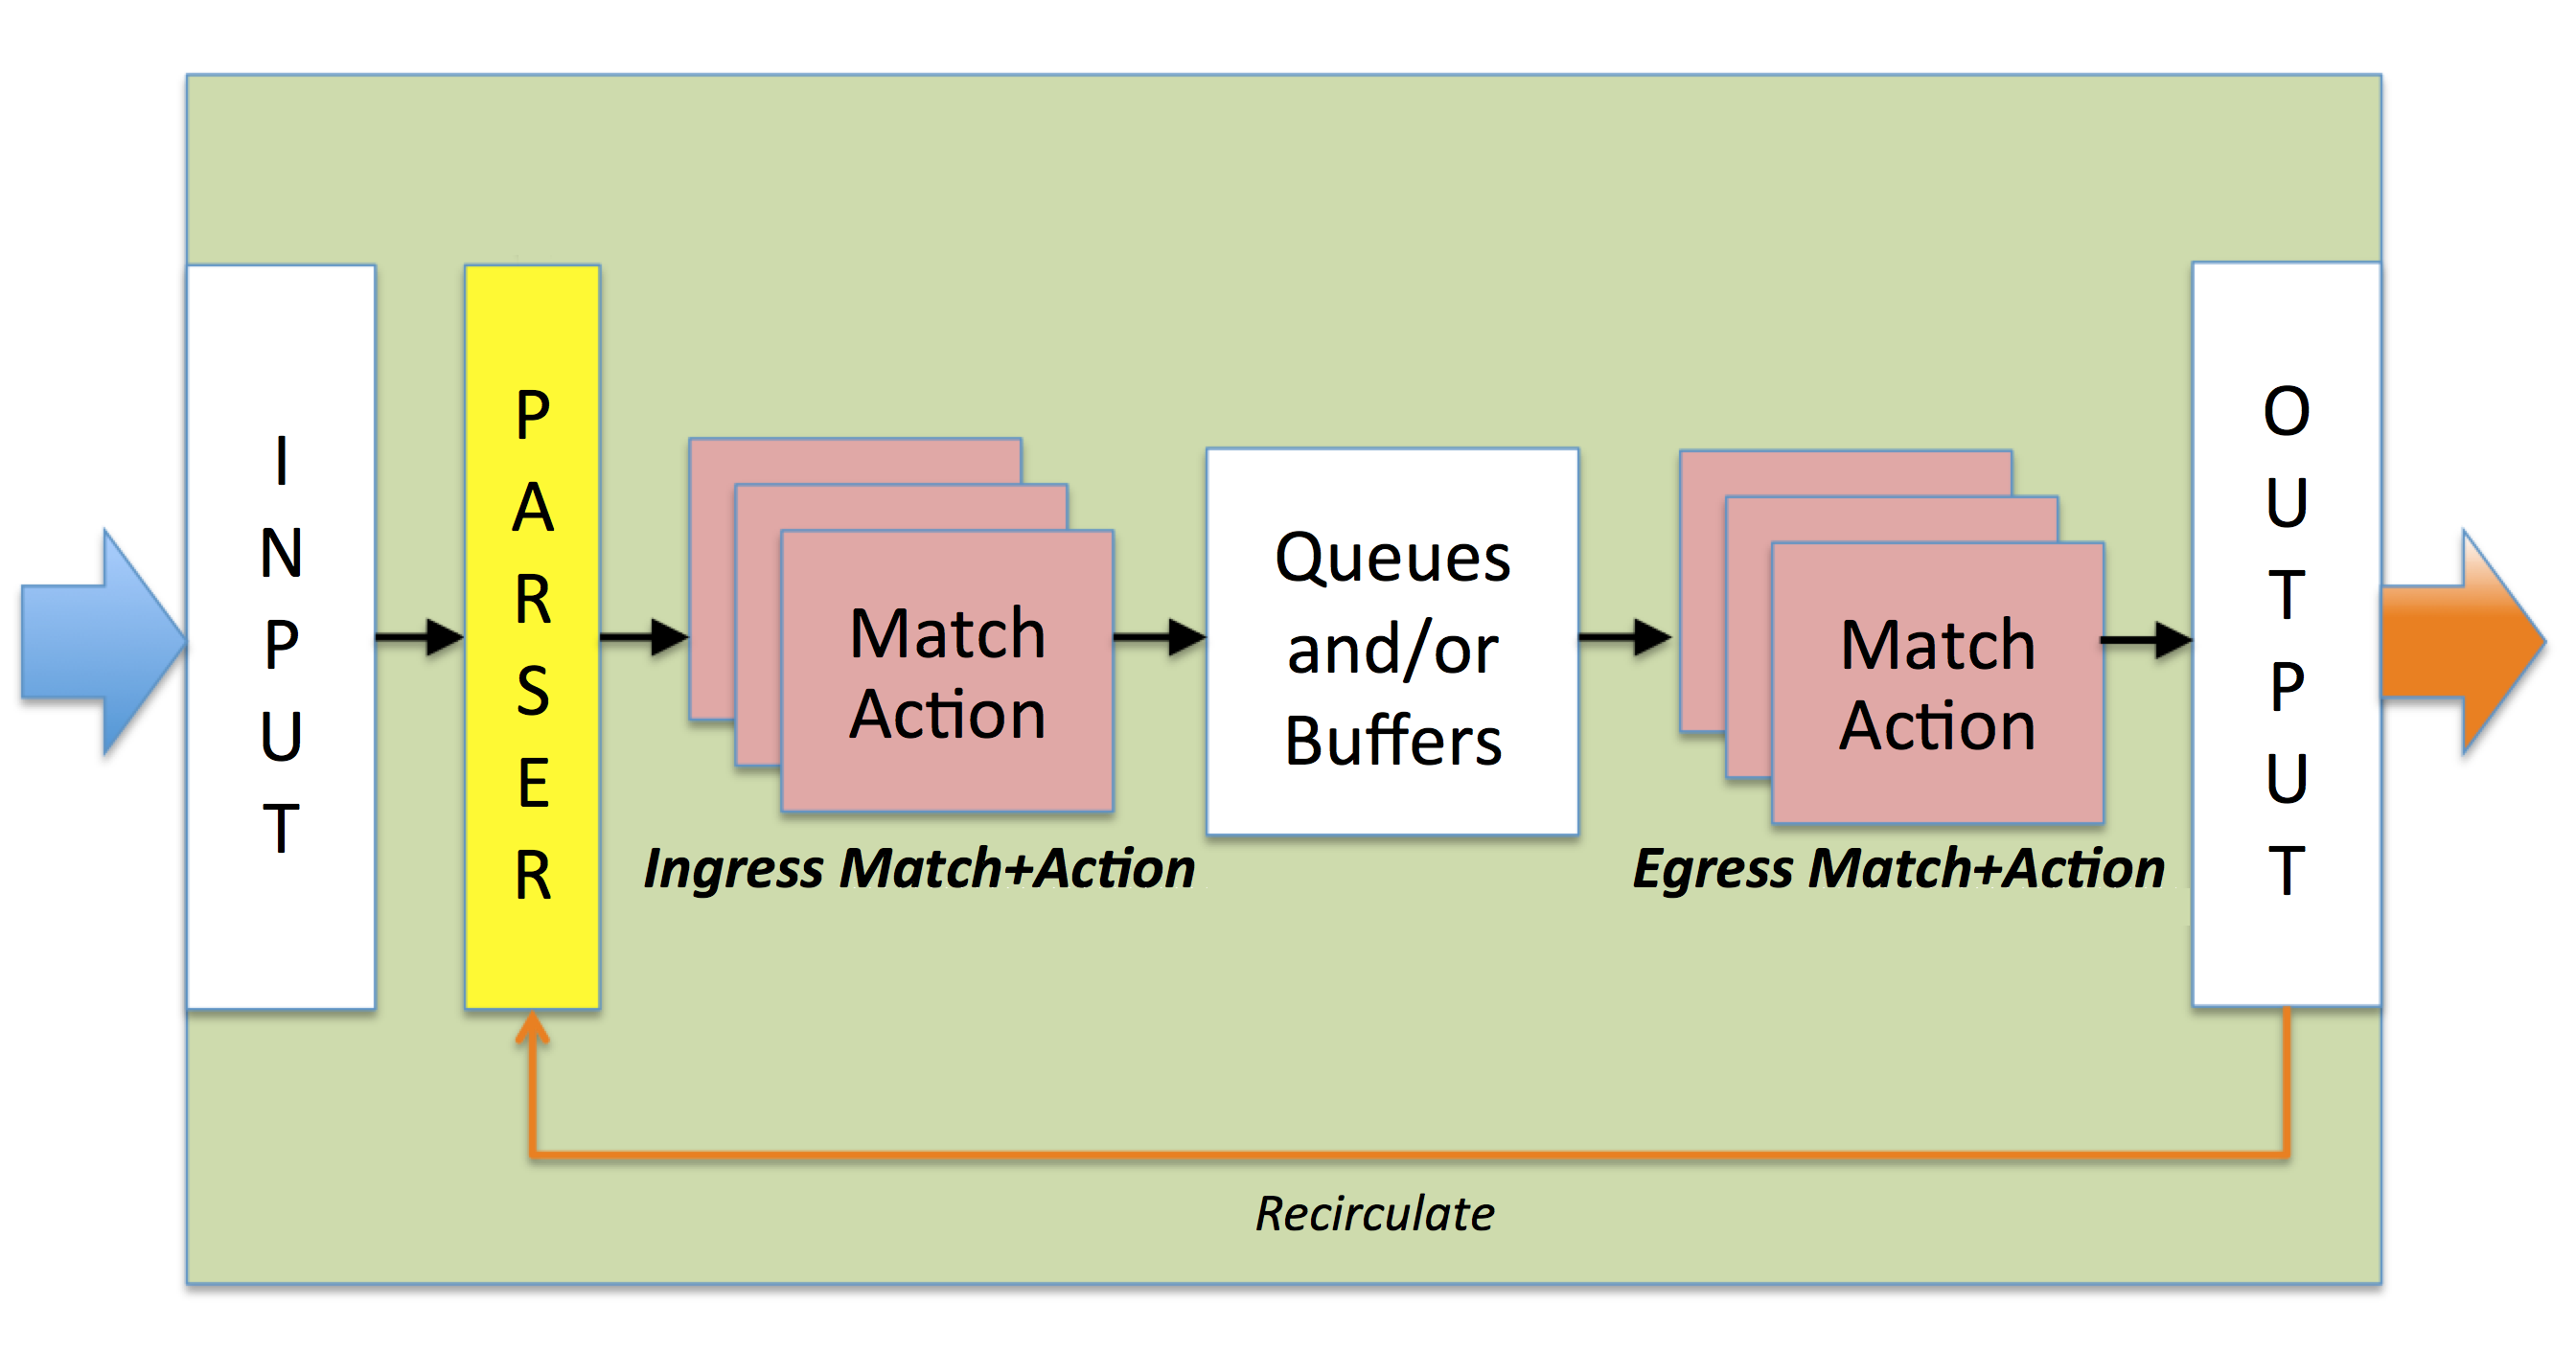
\includegraphics[width=\textwidth]{figures/recirculate.png}
    \caption{Resubmit and Recirculate}
    \label{fig:recirc}
\end{figure}

Figure 5 shows the paths for resubmitting a packet to the parser for
processing.  The top path shows a resubmit process.  The
\texttt{resubmit} action is signalled in the ingress pipeline. Upon
completing that pipeline, the \textbf{original} packet seen on ingress
is resubmitted to the parser along with additional metadata as
specified by the action.  The parser may use the new metadata to make
different parsing decisions than on the original pass through the
parser.

The lower path shows the path for recirculation.  After the packet has
completed both ingress and egress processing, it is deparsed and sent
back to the parser.  The new packet is reparsed, possibly with
metadata preserved from the original packet, and passed to the ingress
pipeline as usual.

For \texttt{resubmit} and \texttt{recirculate}, the
\texttt{instance_type} metadata field distinguishes between first and
later times the packet is being processed.


%%%%%%
%%%%%%
\SECTION{Extern objects}{externs}
%%%%%%
%%%%%%

Although P4 uses \matchaction tables and actions to express basic forwarding
logic, P4 programs might require functionality built out of components
whose behavior is not expressible in P4 itself. Examples of this include
stateful metering operations and parameterizable hash calculations. For this
purpose, P4 allows the specification of extern object types that the
user can instantiate in their P4 program.

Extern types are provided by both standardized and target-specific libraries.
P4 programmers are not intended to define their own extern types, so much
as use the set of supported extern types as a palette of components from which
to compose their programs. 

\SUBSECTION{Extern types}{externtypes} An extern type definition is intended to be 
used by both the programmer and compiler front-end to specify how extern
instances of that type must be instantiated and where they may be used.

An extern type may specify both attributes and methods. Attributes are
properties of the extern object that are bound inside the object
instantiation. Methods are functions that can be called on a given extern
instance at various places in the P4 program.

%%bnf
\begin{lstlisting}[style=BNFstyle]
extern_type_declaration ::= 
    extern_type type_name {
        member_declaration*
    }

member_declaration ::= attribute_declaration | method_declaration

method_declaration ::= 
    method method_name ( method_param_list );

method_param_list ::= method_param [, method_param]*
method_param ::= param_qualifier* type_spec param_name

attribute_declaration ::= 
    attribute attribute_name {
        type : attribute_type ;
        [ optional ; ]
    }

identifier_list ::= variable_name ;

attribute_type ::=  type_spec
\end{lstlisting}
%%endbnf

The extern type indicates that the P4 programmer can instantiate objects of
type \textit{type_name}. Each attribute declaration inside the extern type 
indicates an attribute its instances contain, and the attribute's expected type.

Attributes marked with the \textit{optional} property are not required to
appear in object instantiations, though the compiler backend may impose further
rules as to when an attribute truly is or is not optional.

Each method declaration inside the extern type indicates a method that can be
called on its instances, with standard \textit{object.method(parameters)} 
notation. Methods may have optional parameters, but may not be overloaded (that
is, method names within an extern type must be unique).

While a P4 \textit{extern_type} object describes the interface by which a
extern instance interacts with the code around it, it (by design) does not
express anything about the object's actual behavior. For target-specific
libraries of extern types, human language documentation is likely sufficient 
to fully specify an extern's behavior. For standardized libraries, however,
it is \textit{strongly} recommended that the P4 extern_type is accompanied
with pseudocode written in a general-purpose programming language to rigorously 
document the behavior and semantics of the type and its methods.

\SUBSECTION{Extern Instances}{externinstances}

The P4 programmer can declare instances of these extern types the same way they
declare tables and other standard P4 objects.

%%bnf
\begin{lstlisting}[style=BNFstyle]
extern_instance_declaration ::= 
    extern type_name instance_name ; |
    extern type_name instance_name { 
        extern_attribute_binding +
    }

extern_attribute_binding ::=
    attribute_name : object_ref ;

extern_method_call ::= 
    object_ref . method_name ( arg_list )
\end{lstlisting}
%%endbnf

Method calls must include arguments for all parameters specified by the
object interface. If the method includes any optional parameters, their
arguments may follow the required arguments (similar to optional arguments
in primitive actions).


%%%%%%
%%%%%%
\SECTION{Appendices}{append}
%%%%%%
%%%%%%

\SUBSECTION{Errata}{errata}

TODO

\SUBSECTION{Programming Conventions}{progconventions}

The following is a list of conventions suggested for P4 programs.

\begin{itemize}
\item
Parsing begins with the parser state function named \texttt{start}.
\item
Control flow begins with the control function \texttt{ingress}.
\end{itemize}The following is a list of conventions suggested for P4 programs.

\SUBSECTION{Revision History}{revhistory}

\begin{table}[H]
\begin{center}
\begin{tabular}{| l | l | p{.6\textwidth} |} \hline
\textbf{Release} &
\textbf{Release Date} &
\textbf{Summary of Changes} \\  \hline
1.0.0-rc1 & 2014-09-08 & First public version. \\  \hline
1.0.0-rc2 & 2014-09-09 & Minor typos. \\  \hline
1.0.0-rc3 & 2014-12-30 & Fixed some missing tildes (negations). Drop in parser is now \texttt{parser_drop}. Added \texttt{add} primitive action. Added errata section. \\  \hline
1.0.1 & 2015-01-28 & Added action profiles and action selectors. Added attribute \texttt{support_timeout} to tables. \\  \hline
1.0.2 & 2015-03-03 & Added \texttt{push} and \texttt{pop} primitive actions. \\  \hline
1.1.0-rc1 & - & Added types, typed signatures, and externs. \\  \hline 
\underline{TODO: add more} \\ \hline
\end{tabular}
\end{center}
\caption{Revision History}
\label{tab:revhistory}
\end{table}


\SUBSECTION{Terminology (Incomplete)}{terms}

\begin{table}[H]
\begin{center}
\begin{tabular}{| l | p{.7\textwidth} |} \hline
\textbf{Term} &
\textbf{Definition} \\ \hline
Control Flow &
The logic that selects which tables are applied to a packet when it is processed by a pipeline.  Used to resolve order dependencies. \\ \hline
Egress Queuing &
An abstract P4 functional block logically separating ingress and egress processing. Implementations may expose queuing and buffer resource management interfaces for this block, but this not specified by P4. \\ \hline
Egress Specification &
Metadata set by the ingress pipeline which determines the set of destination ports (and number of instances on each port) to which the packet should be sent  \\ \hline
Order Dependency &
A sequence of match and action operations whose result depends on the order of execution. For example, one table may set a field which another table uses for a match. The control flow is used to determine which of the possible effects is intended. \\ \hline
Parsed Representation &
A representation of a packet's header as a set of header instances, each of which is composed of fields. \\ \hline
Parser &
A functional block which maps a packet to a Parsed Representation \\ \hline
Pipeline &
A sequence of \matchaction tables.  \\ \hline
Run time &
When a switch is processing packets. This is distinguished from configuration time, though these operations may occur at the same time in some implementations. \\ \hline
\end{tabular}
\end{center}
\caption{Terminology}
\label{tab:terminology}
\end{table}

\SUBSECTION{Summary of P4 BNF}{bnfsummary}

%%bnf
\begin{lstlisting}[style=BNFstyle]
p4_program ::= p4_declaration +

p4_declaration ::=
    header_type_declaration | 
    header_instance_declaration |
    field_list_declaration |
    field_list_calculation_declaration |
    calculated_field_declaration |
    value_set_declaration |
    parser_function_declaration |
    parser_exception_declaration |
    counter_declaration |
    meter_declaration |
    register_declaration |
    primitive_action_declaration |
    action_function_declaration |
    action_profile_declaration |
    action_selector_declaration |
    table_declaration |
    extern_type_declaration |
    extern_instance_declaration |
    control_function_declaration |
const_value ::=
    bool_value |
    [ "+" | - ] [ width_spec ] unsigned_value

unsigned_value ::= 
    binary_value | 
    decimal_value | 
    hexadecimal_value

bool_value ::= true | false
binary_value ::=  binary_base binary_digit+
decimal_value ::= decimal_digit+
hexadecimal_value ::= hexadecimal_base hexadecimal_digit+

binary_base ::= 0b | 0B
hexadecimal_base ::= 0x | 0X

binary_digit ::= _ | 0 | 1
decimal_digit ::= binary_digit | 2 | 3 | 4 | 5 | 6 | 7 | 8 | 9
hexadecimal_digit ::= 
    decimal_digit | a | A | b | B | c | C | d | D | e | E | f | F

width_spec ::= decimal_digit+ [ w | s ]
field_value ::= const_value

type_spec ::=
    header [ header_type_name ] |
    metadata [ header_type_name ] |
    field_list |
    field_list_calculation |
    parser |
    parser_exception |
    parser_value_set |
    counter |
    meter |
    register |
    action |
    action_profile |
    table |
    control |
    extern [ extern_type_name ] |
    data_type

data_type ::=
    bit |
    bit < decimal_digit+ > |
    varbit < decimal_digit+ > |
    int < decimal_digit+ >
object_ref ::=
    instance_name |
    header_ref |
    field_ref

general_expr ::= 
    bool_expr | arith_expr | object_ref

bool_expr ::=
    valid ( object_ref ) | bool_expr bool_op bool_expr |
    not bool_expr | ( bool_expr ) | arith_expr rel_op arith_expr |
    bool_value

arith_expr ::=
    object_ref | value | 
    max ( arith_expr , arith_expr ) | min ( arith_expr , arith_expr ) |
    ( arith_expr ) | arith_expr bin_op arith_expr | un_op arith_expr |
    ( data_type ) arith_expr

bin_op ::= "+" | "*" | - | << | >> | & | "|" | ^
un_op ::= ~ | -
bool_op ::= or | and
rel_op ::= > | >= | == | <= | < | !=

header_type_declaration ::= 
   header_type header_type_name { header_dec_body }

header_dec_body ::=
    fields { field_dec * }
    [ length : length_exp ; ]

field_dec ::= data_type field_name ;
length_bin_op ::= "+" | - | "*" | << | >>
length_exp ::=
    const_value |
    field_name |
    length_exp length_bin_op length_exp |
    ( length_exp )

header_instance_declaration ::= header_instance | metadata_instance
header_instance ::= scalar_instance | array_instance
scalar_instance ::= header header_type_name instance_name ;
array_instance ::=
    header header_type_name 
        instance_name "[" const_value "]" ;

metadata_instance ::= 
   metadata header_type_name
       instance_name [ metadata_initializer ] | ;

metadata_initializer ::= { [ field_name : field_value ; ] + }
header_ref ::= header_instance_name | header_instance_name "[" index "]"
index ::= const_value | last | next

field_ref ::= header_ref . field_name
field_list_declaration ::=
    field_list field_list_name {
        [ field_list_entry ; ] *
    }

field_list_entry ::= 
    object_ref | field_value
field_list_calculation_declaration ::=
    field_list_calculation field_list_calculation_name {
        input {
            [ field_list_name ; ] +
        }
        algorithm : stream_function_algorithm_name ;
        output_width : const_value ;
    }
calculated_field_declaration ::=
    calculated_field field_ref { update_verify_spec + }

update_verify_spec ::=
    update_or_verify field_list_calculation_name [ if_cond ] ;

update_or_verify ::= update | verify
if_cond ::= if ( calc_bool_cond )
calc_bool_cond ::=
    valid ( header_ref | field_ref ) |
    field_ref == field_value
value_set_declaration ::= parser_value_set value_set_name;
parser_function_declaration ::=
    parser parser_state_name { parser_function_body }

parser_function_body ::=
    parser_body_call*
    return_statement

parser_body_call ::=
    extract_statement |
    set_statement |
    extern_method_call ;

extract_statement ::= extract ( header_extract_ref ); 
header_extract_ref ::=
     header_instance_name |
     header_instance_name "[" header_extract_index "]"

header_extract_index ::= const_value | next

set_statement ::= set_metadata ( field_ref, general_expr ) ;

return_statement ::=
    return_value_type |
    return select ( select_exp ) { case_entry + }

return_value_type ::= 
    return parser_state_name ; | 
    return control_function_name ; | 
    parse_error parser_exception_name ;

case_entry ::= value_list : case_return_value_type ;
value_list ::= value_or_masked [ , value_or_masked ]* | default

case_return_value_type ::= 
    parser_state_name | 
    control_function_name | 
    parse_error parser_exception_name

value_or_masked ::=
    field_value | field_value mask field_value | value_set_name |
    ( value_or_masked [, value_or_masked] * )
 
select_exp ::= field_or_data_ref [, field_or_data_ref] * 
field_or_data_ref ::=
    field_ref |
    latest.field_name |
    current( const_value , const_value )
parser_exception_declaration ::=
    parser_exception parser_exception_name {
        set_statement *
        return_or_drop ;
    }

return_or_drop ::= return_to_control | parser_drop
return_to_control ::= return control_function_name
counter_declaration ::=
    counter counter_name { 
        type : counter_type ;
        [ direct_or_static ; ]
        [ instance_count : const_value ; ]
        [ min_width : const_value ; ]
        [ saturating ; ]
    }

counter_type ::= bytes | packets
direct_or_static ::= direct_attibute | static_attribute
direct_attribute ::= direct : table_name
static_attribute ::= static : table_name
meter_declaration ::= 
    meter meter_name {
        type : meter_type ;
        result : field_ref ;
        [ direct_or_static ; ]
        [ instance_count : const_value ; ]
    }

meter_type ::= bytes | packets
register_declaration ::= 
    register register_name {
        width_or_layout ;
        [ direct_or_static ; ]
        [ instance_count : const_value ; ]
        [ attribute_list ; ]
    }

width_or_layout ::= width_declaration | layout_declaration
width_declaration ::= width : const_value ;
layout_declaration ::= layout : header_type_name ;

attribute_list ::= attributes : attr_entry
attr_entry ::= signed | attr_entry , attr_entry
register_ref ::=
    register_name "[" const_value "]" [.field_name]
primitive_action_declaration ::= 
    primitive_action action_name ( [ simple_param_list ] ) ;

simple_param_list ::= param_name [, param_name]*
compound_action_function_declaration ::=
    action action_name ( [ action_param_list ] ) { action_statement + } |
    action action_name ( [ action_param_list ] ) ;

action_param_list ::= action_param [, action_param]*
action_param ::= param_qualifier* data_type param_name

param_qualifier ::= in | inout

action_statement ::= 
    action_name ( [ arg_list ] ) ; |
    extern_method_call ;

arg_list ::= general_expr [, general_expr]*
action_profile_declaration ::=
    action_profile action_profile_name {
        action_specification
        [ size : const_value ; ]
	[ dynamic_action_selection : selector_name ; ]
    }

action_specification ::= 
    actions { [ action_name ] + }

action_selector_declaration ::=
    action_selector selector_name {
        selection_key : field_list_calculation_name ;
    }
table_declaration ::=
    table table_name {
        [ reads { field_match + } ]
        table_actions
        [ min_size : const_value ; ]
        [ max_size : const_value ; ]
        [ size : const_value ; ]
	[ support_timeout : bool_value ; ]
    }

field_match ::= field_or_masked_ref : field_match_type ;
field_or_masked_ref ::= 
    header_ref | field_ref | field_ref mask const_value

field_match_type ::= exact | ternary | lpm | range | valid

table_actions ::= 
    action_specification | action_profile_specification

action_specification ::= 
    actions { [ action_name ; ] + }

action_profile_specification ::= 
    action_profile : action_profile_name
control_function_declaration ::=
    control control_fn_name control_block
control_block ::= { control_statement * }
control_statement ::= 
    apply_call |
    apply_and_select_block |
    extern_method_call ; |
    if_else_statement |
    control_fn_name ( ) ; |
    return ;

apply_call ::= apply ( table_name ) ;
apply_and_select_block ::= apply ( table_name ) { [ case_list ] }
case_list ::= action_case + | hit_miss_case +
action_case ::= action_or_default control_block
action_or_default ::= action_name | default
hit_miss_case ::= hit_or_miss control_block
hit_or_miss ::= hit | miss

if_else_statement ::=
    if ( bool_expr ) control_block
    [ else_block ]

else_block ::= else control_block | else if_else_statement
extern_type_declaration ::= 
    extern_type type_name {
        member_declaration*
    }

member_declaration ::= attribute_declaration | method_declaration

method_declaration ::= 
    method method_name ( method_param_list );

method_param_list ::= method_param [, method_param]*
method_param ::= param_qualifier* type_spec param_name

attribute_declaration ::= 
    attribute attribute_name {
        type : attribute_type ;
        [ optional ; ]
    }

identifier_list ::= variable_name ;

attribute_type ::=  type_spec
extern_instance_declaration ::= 
    extern type_name instance_name ; |
    extern type_name instance_name { 
        extern_attribute_binding +
    }

extern_attribute_binding ::=
    attribute_name : object_ref ;

extern_method_call ::= 
    object_ref . method_name ( arg_list )

\end{lstlisting}
%%endbnf

\SUBSECTION{P4 Reserved Words}{reservedwords}

The following are reserved words in P4 and should not be used as 
identifiers.\footnote{There is an open issue whether all P4 keywords 
will in fact be reserved.}

\begin{Verbatim}[commandchars=\\\{\}]
action
action_function_declaration
action_profile
action_selector
algorithm
and
apply
attribute
attributes
bit
bytes
calculated_field
control
counter
direct
direct_attibute
dynamic_action_selection
else
extern
extern_type
extract
false
field_list
field_list_calculation
fields
header
header_type
hit
if
in
inout
input
instance_count
int
last
layout
mask
max
metadata
meter
method
min
min_width
miss
next
not
optional
or
output_width
packets
parse_error
parser
parser_drop
parser_exception
parser_value_set
primitive_action
range
register
result
return
saturating
select
selection_key
set_metadata
signed
static
table
true
update
valid
value
varbit
verify
width
\end{Verbatim}

\SUBSECTION{Examples}{examples}

\SUBSUBSECTION{The Annotated mTag Example}{mtagexample}

This section presents the mTag example. The example describes two separate 
P4 programs, mtag-edge and mtag-aggregation, as described in the introduction 
in Section~\ref{sec:mtag}.

The code is written in P4 whose syntax allows the application of a C preprocessor 
to P4 files. Thus directives such as \texttt{\#define} and \texttt{\#include} are used in 
the program with the same effects as if writing C code. This is a convention 
used by these examples; the P4 language does not mandate this syntax.

The example code is split into the following files

\begin{itemize}
\item
\texttt{headers.p4}: The declaration of all header types used in both programs.
\item
\texttt{parser.p4}: The parser program shared by both programs.
\item
\texttt{actions.p4}: Common actions used by both programs.
\item
\texttt{mtag-edge.p4}: The main program for the edge switch
\item
\texttt{mtag-aggregation.p4}: The main program for any aggregation switch
\end{itemize}

The full source for all files is provided on the P4 website [2].

We start with \texttt{header.p4}. 

% For code listings: http://en.wikibooks.org/wiki/LaTeX/Source_Code_Listings

%%code
\begin{lstlisting}[style=P4style]
////////////////////////////////////////////////////////////////
// Header type definitions
////////////////////////////////////////////////////////////////

// Standard L2 Ethernet header
header_type ethernet_t {
    fields {
        bit<48> dst_addr;
        bit<48> src_addr;
        bit<16> ethertype;
    }
}

// Standard VLAN tag
header_type vlan_t {
    fields {
        bit<3>  pcp;
        bit     cfi;
        bit<12> vid;
        bit<16> ethertype;
    }
}

// The special m-tag used to control forwarding through the
// aggregation layer of  data center
header_type mTag_t {
    fields {
        bit<8>  up1;
        bit<8>  up2;
        bit<8>  down1;
        bit<8>  down2;
        bit<16> ethertype;
    }
}

// Standard IPv4 header
header_type ipv4_t {
    fields {
        bit<4> version;
        bit<4> ihl;
        bit<8> diffserv;
        bit<16> totalLen;
        bit<16> identification;
        bit<3> flags;
        bit<13> fragOffset;
        bit<8> ttl;
        bit<8> protocol;
        bit<16> hdrChecksum;
        bit<32> srcAddr;
        bit<32> dstAddr;
        varbit<320> options;
    }
    length : ihl * 4;
}

// Assume standard metadata from compiler.

// Define local metadata here.
//
// copy_to_cpu is an example of target specific intrinsic metadata
// It has special significance to the target resulting in a
// copy of the packet being forwarded to the management CPU.

header_type local_metadata_t {
    fields {
        bit<16> cpu_code        // Code for packet going to CPU
        bit<4> port_type        // Type of port: up, down, local...
        bit ingress_error       // An error in ingress port check
        bit was_mtagged         // Track if pkt was mtagged on ingr
        bit copy_to_cpu         // Special code resulting in copy to CPU
        bit bad_packet          // Other error indication
        bit<8> color            // For metering
    }
}
\end{lstlisting}
%%endcode

The parser function shared by the programs is as follows.

%%code
\begin{lstlisting}[style=P4style]
////////////////////////////////////////////////////////////////
// Parser functions and related definitions
////////////////////////////////////////////////////////////////

////////////////////////////////////////////////////////////////
// Header instance definitions
//
// Header instances are usually defined with the parser as
// that is where they are initialized.
//
////////////////////////////////////////////////////////////////

header ethernet_t ethernet;
header vlan_t vlan;
header mTag_t mtag;
header ipv4_t ipv4;

// Local metadata instance declaration
metadata local_metadata_t local_metadata;

////////////////////////////////////////////////////////////////
// Parser state machine description
////////////////////////////////////////////////////////////////

// Start with ethernet always.
parser start {
    return ethernet;    
}

parser ethernet {
    extract(ethernet);   // Start with the ethernet header
    return select(latest.ethertype) {
        0x8100:     vlan;
        0x800:      ipv4;
        default:    ingress;
    }
}

// Extract the VLAN tag and check for an mTag
parser vlan {
    extract(vlan);
    return select(latest.ethertype) {
        0xaaaa:     mtag;
        0x800:      ipv4;
        default:    ingress;
    }
}

// mTag is allowed after a VLAN tag only (see above)
parser mtag {
    extract(mtag);
    return select(latest.ethertype) {
        0x800:      ipv4;
        default:    ingress;
    }
}

parser ipv4 {
    extract(ipv4);
    return ingress;  // All done with parsing; start matching
}
\end{lstlisting}
%%endcode

Here are the common actions for the two programs.

%%code
\begin{lstlisting}[style=P4style]
////////////////////////////////////////////////////////////////
//
// actions.p4
//
// This file defines the common actions that can be exercised by
// either an edge or an aggregation switch. 
//
////////////////////////////////////////////////////////////////

////////////////////////////////////////////////////////////////
// Actions used by tables
////////////////////////////////////////////////////////////////

// Copy the packet to the CPU;
action common_copy_pkt_to_cpu(in bit<8> cpu_code, in bit bad_packet) {
    modify_field(local_metadata.copy_to_cpu, 1);
    modify_field(local_metadata.cpu_code, cpu_code);
    modify_field(local_metadata.bad_packet, bad_packet);
}

// Drop the packet; optionally send to CPU and mark bad
action common_drop_pkt(in bit do_copy, in bit<8> cpu_code, in bit bad_packet) {
    modify_field(local_metadata.copy_to_cpu, do_copy);
    modify_field(local_metadata.cpu_code, cpu_code);
    modify_field(local_metadata.bad_packet, bad_packet);
    drop();
}

// Set the port type; see run time mtag_port_type. 
// Allow error indication.
action common_set_port_type(in bit<4> port_type, in bit ingress_error) {
    modify_field(local_metadata.port_type, port_type);
    modify_field(local_metadata.ingress_error, ingress_error);
}
\end{lstlisting}
%%endcode

Here are excerpts from the edge program.

%%code
\begin{lstlisting}[style=P4style]
////////////////////////////////////////////////////////////////
//
// mtag-edge.p4
//
// This file defines the behavior of the edge switch in an mTag
// example.
//
//
////////////////////////////////////////////////////////////////

// Include the header definitions and parser
// (with header instances)
#include "headers.p4"
#include "parser.p4"
#include "actions.p4"  // For actions marked "common_"

#define PORT_COUNT 64  // Total ports in the switch

////////////////////////////////////////////////////////////////
// Table definitions
////////////////////////////////////////////////////////////////

// Remove the mtag for local processing/switching
action _strip_mtag() {
    // Strip the tag from the packet...
    remove_header(mtag);
    // but keep state that it was mtagged.
    modify_field(local_metadata.was_mtagged, 1);
}

// Always strip the mtag if present on the edge switch
table strip_mtag {
    reads {
        mtag     : valid; // Was mtag parsed?
    }
    actions {
        _strip_mtag;      // Strip mtag and record metadata
        no_op;            // Pass thru otherwise
    }
}

////////////////////////////////////////////////////////////////

// Identify ingress port: local, up1, up2, down1, down2
table identify_port {
    reads {
        standard_metadata.ingress_port : exact;
    }
    actions { // Each table entry specifies *one* action
        common_set_port_type;
        common_drop_pkt;        // If unknown port
        no_op;         // Allow packet to continue
    }
    max_size : 64; // One rule per port
}

. . .  // Removed code related to local switching

// Add an mTag to the packet; select egress spec based on up1
action add_mTag(in bit<8> up1, in bit<8> up2, 
                in bit<8> down1, in bit<8> down2) {
    add_header(mtag);
    // Copy VLAN ethertype to mTag
    modify_field(mtag.ethertype, vlan.ethertype);

    // Set VLAN's ethertype to signal mTag
    modify_field(vlan.ethertype, 0xaaaa);

    // Add the tag source routing information
    modify_field(mtag.up1, up1);
    modify_field(mtag.up2, up2);
    modify_field(mtag.down1, down1);
    modify_field(mtag.down2, down2);

    // Set the destination egress port as well from the tag info
    modify_field(standard_metadata.egress_spec, up1);
}

// Count packets and bytes by mtag instance added
counter pkts_by_dest {
    type : packets;
    direct : mTag_table;
}

counter bytes_by_dest {
    type : bytes;
    direct : mTag_table;
}

// Check if the packet needs an mtag and add one if it does.
table mTag_table {
    reads {
        ethernet.dst_addr    : exact;
        vlan.vid             : exact;
    }
    actions {
        add_mTag;  // Action called if pkt needs an mtag.
        // Option: If no mtag setup, forward to the CPU
        common_copy_pkt_to_cpu;
        no_op;
    }
    max_size                 : 20000;
}

// Packets from agg layer must stay local; enforce that here
table egress_check {
    reads {
        standard_metadata.ingress_port : exact;
        local_metadata.was_mtagged : exact;
    }

    actions {    
        common_drop_pkt;
        no_op;
    }
    max_size : PORT_COUNT; // At most one rule per port
}

// Egress metering; this could be direct, but we let SW 
// use whatever mapping it might like to associate the
// meter cell with the source/dest pair
meter per_dest_by_source {
    type : bytes;
    result : local_metadata.color;
    instance_count : PORT_COUNT * PORT_COUNT;  // Per source/dest pair
}

action meter_pkt(in int<12> meter_idx) {
    meter(per_dest_by_source, meter_idx, local_metadata.color);
}
        
// Mark packet color, for uplink ports only
table egress_meter {
    reads {
        standard_metadata.ingress_port : exact;
        mtag.up1 : exact;
    }
    actions {
        meter_pkt;
        no_op;
    }
    size : PORT_COUNT * PORT_COUNT;  // Could be smaller
}

// Apply meter policy
counter per_color_drops {
    type : packets;
    direct : meter_policy;
}

table meter_policy {
    reads {
        metadata.ingress_port : exact;
        local_metadata.color : exact;
    }
    actions {
        drop; // Automatically counted by direct counter above
        no_op;
    }
    size : 4 * PORT_COUNT;
}


////////////////////////////////////////////////////////////////
// Control function definitions
////////////////////////////////////////////////////////////////

// The ingress control function
control ingress {

    // Always strip mtag if present, save state
    apply(strip_mtag);

    // Identify the source port type
    apply(identify_port);

    // If no error from source_check, continue
    if (local_metadata.ingress_error == 0) {
        // Attempt to switch to end hosts
        apply(local_switching); // not shown; matches on dest addr

        // If not locally switched, try to setup mtag
        if (standard_metadata.egress_spec == 0) {
            apply(mTag_table);
        }
     }
}

// The egress control function
control egress {
    // Check for unknown egress state or bad retagging with mTag.
    apply(egress_check);

    // Apply egress_meter table; if hit, apply meter policy
    apply(egress_meter) {
        hit {
            apply(meter_policy);
        }
    }
}
\end{lstlisting}
%%endcode

The key table for mtag-aggregation is shown below.

%%code
\begin{lstlisting}[style=P4style]
////////////////////////////////////////////////////////////////
//
// mtag-aggregation.p4
//
////////////////////////////////////////////////////////////////

// Include the header definitions and parser (with header instances)
#include "headers.p4"
#include "parser.p4"
#include "actions.p4"  // For actions marked "common_"

////////////////////////////////////////////////////////////////
// check_mtag table:  
//   Make sure pkt has mtag; Apply drop or to-cpu policy if not
////////////////////////////////////////////////////////////////

table check_mtag { // Statically programmed w/ one entry
. . . // Reads if mtag valid; drop or copy to CPU
}

////////////////////////////////////////////////////////////////
// identify_port table:  
//   Check if up or down facing port as programmed at run time.
////////////////////////////////////////////////////////////////

table identify_port {
. . . // Read ingress_port; call common_set_port_type.
}

////////////////////////////////////////////////////////////////

// Actions to copy the proper field from mtag into the egress spec
action use_mtag_up1() { // This is actually never used on agg switches
    modify_field(standard_metadata.egress_spec, mtag.up1);
}
action use_mtag_up2() {
    modify_field(standard_metadata.egress_spec, mtag.up2);
}
action use_mtag_down1() {
    modify_field(standard_metadata.egress_spec, mtag.down1);
}
action use_mtag_down2() {
    modify_field(standard_metadata.egress_spec, mtag.down2);
}

// Table to select output spec from mtag
table select_output_port {
    reads {
        local_metadata.port_type  : exact; // Up, down, level 1 or 2.
    }
    actions {
        use_mtag_up1;
        use_mtag_up2;
        use_mtag_down1;
        use_mtag_down2;
        // If port type is not recognized, previous policy applied
        no_op; 
    }
    max_size : 4; // Only need one entry per port type
}

////////////////////////////////////////////////////////////////
// Control function definitions
////////////////////////////////////////////////////////////////

// The ingress control function
control ingress {
    // Verify mTag state and port are consistent
    apply(check_mtag);
    apply(identify_port);
    apply(select_output_port);
}

// No egress function used in the mtag-agg example.
\end{lstlisting}
%%endcode

The following is an example header file that might be used with the mtag example 
above. This shows the following:

\begin{itemize}
\item
Type definitions for port types (\texttt{mtag_port_type_t}) meter levels \\
(\texttt{mtag_meter_levels_t}) 
and a table entry handle (\texttt{entry_handle_t}).  
\item
An example function to add an entry to the \texttt{identify_port} table, \\
\texttt{table_identify_port_add_with_set_port_type}. 
The action to use with the entry is indicated at the end of the function name: 
\texttt{set_port_type}.
\item
Functions to set the default action for the identify_port table: \\
\texttt{table_indentify_port_default_common_drop_pkt} and \\
\texttt{table_indentify_port_default_common_set_port_type}.
\item
A function to add an entry to the mTag table: \\
\texttt{table_mTag_table_add_with_add_mTag}
\item
A function to get a counter associated with the meter table: \\
\texttt{counter_per_color_drops_get}.
\end{itemize}

\begin{lstlisting}[language=C,frame=single]
/**
 * Run time header file example for CCR mTag example
 */


#ifndef MTAG_RUN_TIME_H
#define MTAG_RUN_TIME_H

/**
 * @brief Port types required for the mtag example
 *
 * Indicates the port types for both edge and aggregation
 * switches.
 */

typedef enum mtag_port_type_e {
    MTAG_PORT_UNKNOWN,        /* Uninitialized port type */
    MTAG_PORT_LOCAL,          /* Locally switch port for edge */
    MTAG_PORT_EDGE_TO_AG1,    /* Up1: edge to agg layer 1 */
    MTAG_PORT_AG1_TO_AG2,     /* Up2: Agg layer 1 to agg layer 2 */
    MTAG_PORT_AG2_TO_AG1,     /* Down2: Agg layer 2 to agg layer 1 */
    MTAG_PORT_AG1_TO_EDGE,     /* Down1: Agg layer 1 to edge */
    MTAG_PORT_ILLEGAL,        /* Illegal value */
    MTAG_PORT_COUNT
} mtag_port_type_t;

/**
 * @brief Colors for metering
 *
 * The edge switch supports metering from local ports up to the
 * aggregation layer.
 */

typedef enum mtag_meter_levels_e {
    MTAG_METER_COLOR_GREEN,  /* No congestion indicated */
    MTAG_METER_COLOR_YELLOW, /* Above low water mark */
    MTAG_METER_COLOR_RED,    /* Above high water mark */
    MTAG_METER_COUNT
} mtag_meter_levels_t;

typedef uint32_t entry_handle_t;

/* mTag table */

/**
 * @brief Add an entry to the edge identify port table
 * @param ingress_port The port number being identified
 * @param port_type The port type associated with the port
 * @param ingress_error The value to use for the error indication
 */

entry_handle_t table_identify_port_add_with_set_port_type(
    uint32_t ingress_port, 
    mtag_port_type_t port_type,
    uint8_t ingress_error);

/**
 * @brief Set the default action of the identify port
 * table to send the packet to the CPU.
 * @param do_copy Set to 1 if should send copy to the CPU
 * @param cpu_code If do_copy, this is the code used
 * @param bad_packet Set to 1 to flag packet as bad
 *
 * This allows the programmer to say: If port type is not
 * set, this is an error; let me see the packet.
 *
 * Also allows just a drop of the packet.
 */

int table_indentify_port_default_common_drop_pkt(
    uint8_t do_copy,
    uint16_t cpu_code,
    uint8_t bad_packet);

/**
 * @brief Set the default action of the identify port
 * table to set to the given value
 * @param port_type The port type associated with the port
 * @param ingress_error The value to use for the error indication
 *
 * This allows the programmer to say "default port type is local"
 */

int table_indentify_port_default_common_set_port_type(
    mtag_port_type_t port_type,
    uint8_t ingress_error);

/**
 * @brief Add an entry to the add mtag table
 * @param dst_addr The L2 destination MAC for matching
 * @param vid The VLAN ID used for matching
 * @param up1 The up1 value to use in the mTag
 * @param up2 The up2 value to use in the mTag
 * @param down1 The down1 value to use in the mTag
 * @param down2 The down2 value to use in the mTag
 */
entry_handle_t table_mTag_table_add_with_add_mTag(
    mac_addr_t dst_addr, uint16_t vid,
    uint8_t up1, uint8_t up2, uint8_t down1, uint8_t down2);

/**
 * @brief Get the number of drops by ingress port and color
 * @param ingress_port The ingress port being queried.
 * @param color The color being queried.
 * @param count (output) The current value of the parameter.
 * @returns 0 on success.
 */
int counter_per_color_drops_get(
    uint32_t ingress_port,
    mtag_meter_levels_t color,
    uint64_t *count);

#endif /* MTAG_RUN_TIME_H */
\end{lstlisting}

\SUBSUBSECTION{Adding Hysteresis to mTag Metering with Registers}{hysteresis}

In the previous section, the mtag-edge switch used metering between local 
ports and the aggregation layer. Suppose that network simulation indicated 
a benefit if hysteresis could be used with the meters. That is, once the meter 
was red, packets are discarded until the meter returned to green (not just 
to yellow).
This can be achieved by adding a register set parallel to the meters. Each 
cell in the register set holds the "previous" color of the meter. 

Here are the changes to support this feature. The meter index is stored in 
local metadata for convenience.

%%code
\begin{lstlisting}[style=P4style]
////////////////////////////////////////////////////////////////
//
// headers.p4:  Add the meter index to the local metadata.
//
////////////////////////////////////////////////////////////////

header_type local_metadata_t {
    fields {
        bit<16> cpu_code        // Code for packet going to CPU
        bit<4> port_type        // Type of port: up, down, local...
        bit ingress_error       // An error in ingress port check
        bit was_mtagged         // Track if pkt was mtagged on ingr
        bit copy_to_cpu         // Special code resulting in copy to CPU
        bit bad_packet          // Other error indication
        bit<8> color            // For metering
        bit<8> prev_color       // For metering hysteresis
        bit<16> meter_idx       // Index used for metering
    }
}


////////////////////////////////////////////////////////////////
// mtag-edge.p4:  Declare registers and add table to update them
////////////////////////////////////////////////////////////////

// The register stores the "previous" state of the color.
// Index is the same as that used by the meter.
register prev_color {
    width : 8;
    // paired w/ meters above
    instance_count : PORT_COUNT * PORT_COUNT;
}

// Action: Update the color saved in the register
action update_prev_color(in bit<8> new_color) {
    modify_field(prev_color[local_metadata.meter_idx], new_color);
}

// Action: Override packet color with that from the parameter
action mark_pkt(in bit<8> color) {
    modify_field(local_metadata.color, color);
}

// Update meter packet action to save data
action meter_pkt(in int<12> meter_idx) {
    // Save index and previous color in packet metadata
    modify_field(local_metadata.meter_idx, meter_idx);
    modify_field(local_metadata.prev_color, prev_color[meter_idx]);
    meter(per_dest_by_source, meter_idx, local_metadata.color);
}


//
// This table is statically populated with the following rules:
//    color: green,  prev_color: red    ==> update_prev_color(green)
//    color: red,    prev_color: green  ==> update_prev_color(red)
//    color: yellow, prev_color: red    ==> mark_pkt(red)
// Otherwise, no-op.
//
table hysteresis_check {
    reads {
        local_metadata.color : exact;
        local_metadata.prev_color : exact;
    }
    actions {
        update_prev_color;
        mark_pkt;
        no_op;
    }
    size : 4;
}

////////////////////////////////////////////////////////////////
// In the egress control function, check for hysteresis
////////////////////////////////////////////////////////////////

control egress {
    // Check for unknown egress state or bad retagging with mTag.
    apply(egress_check);
    apply(egress_meter) {
        hit {
            apply(hysteresis_check);
            apply(meter_policy);
        }
    }
}
\end{lstlisting}
%%endcode


\SUBSUBSECTION{ECMP Selection Example}{ecmpselection}

This example shows how ECMP can be implemented using an action profile with
action selector.

%%code
\begin{lstlisting}[style=P4style]
table ipv4_routing {
    reads {
        ipv4.dstAddr: lpm;
    }
    action_profile : ecmp_action_profile;
    size : 16384;    // 16K possible IPv4 prefixes
}

action_profile ecmp_action_profile {
    actions {
        nhop_set;
        no_op;
    }
    size : 4096;    // 4K possible next hops
    dynamic_action_selection : ecmp_selector;
}

// list of fields used to determine the ECMP next hop
field_list l3_hash_fields {
    ipv4.srcAddr;
    ipv4.dstAddr;
    ipv4.protocol;
    ipv4.protocol;
    tcp.sport;
    tcp.dport;
}

field_list_calculation ecmp_hash {
    input {
        l3_hash_fields;
    }
    algorithm : crc16;
    output_width : 16;
}

action_selector ecmp_selector {
    selection_key : ecmp_hash;
}
\end{lstlisting}
%%endcode

\SUBSECTION{References}{references}

[1] Bosshart, et al. \textit{P4: Programming Protocol-Independent Packet Processors}. 
Computer Communication Review, July 2014.  \url{http://www.sigcomm.org/ccr/papers/2014/July/0000000.0000004}.

[2] The P4 Language Consortium web site. \url{http://www.p4.org}.

\end{document}
